% In questo file vengono definiti comandi (macro) utili in tutti i documenti

\newcommand{\gruppo}{\textit{Sirius}} % nome gruppo
\newcommand{\progetto}{\textit{Sequenziatore}} % nome progetto
\newcommand{\capitolato}{\href{http://www.math.unipd.it/~tullio/IS-1/2013/Progetto/C4p.pdf}{http://www.math.unipd.it/~tullio/IS-1/2013/Progetto/C4p.pdf}} 

% GLOSSARIO
\newcommand{\lastversionG}{4.0.0}
\newcommand{\Glossario}{\textit{Glossario\_{}v\lastversionG{}.pdf}}
\newcommand{\doctitleG}{Glossario}
\newcommand{\infoG}{\doctitleG\ v\lastversionG}

% NORME DI PROGETTO
\newcommand{\lastversionNDP}{4.0.0}
\newcommand{\NormeDiProgetto}{\textit{NormeDiProgetto\_{}v\lastversionNDP{}.pdf}}
\newcommand{\doctitleNDP}{Norme di progetto}
\newcommand{\infoNDP}{\doctitleNDP\ v\lastversionNDP}

% ANALISI DEI REQUISITI
\newcommand{\lastversionAR}{3.0.0}
\newcommand{\AnalisiDeiRequisiti}{\textit{AnalisiDeiRequisiti\_{}v\lastversionAR{}.pdf}}
\newcommand{\doctitleAR}{Analisi dei requisiti}
\newcommand{\infoAR}{\doctitleAR\ v\lastversionAR}

% Studio di fattibilita
\newcommand{\lastversionSDF}{2.0.0}
\newcommand{\StudioDiFattibilita}{\textit{StudioDiFattibilita\_{}v\lastversionSDF{}.pdf}}
\newcommand{\doctitleSDF}{Studio Di Fattibilità}
\newcommand{\infoSDF}{\doctitleSDF\ v\lastversionSDF}

% Piano di qualifica
\newcommand{\lastversionPDQ}{4.0.0}
\newcommand{\PianoDiQualifica}{\textit{PianoDiQualifica\_{}v\lastversionPDQ{}.pdf}}
\newcommand{\doctitlePDQ}{Piano Di Qualifica}
\newcommand{\infoPDQ}{\doctitlePDQ\ v\lastversionPDQ}

% VERBALE 2014-02-03
\newcommand{\lastversionVb}{2.0.0}
\newcommand{\VerbaleB}{\textit{Verbale2014-02-03\_{}v\lastversionVb{}.pdf}}
\newcommand{\doctitleVb}{Verbale 2014-02-03}
\newcommand{\infoVb}{\doctitleVb\ v\lastversionVb}

% VERBALE 2014-07-20
\newcommand{\lastversionVN}{1.0.0}
\newcommand{\VerbaleN}{\textit{Verbale2014-07-20\_{}v\lastversionVN{}.pdf}}
\newcommand{\doctitleVN}{Verbale 2014-07-20}
\newcommand{\infoVN}{\doctitleVN\ v\lastversionVN}

%Piano di progetto
\newcommand{\lastversionPDP}{4.0.0}
\newcommand{\PianoDiProgetto}{\textit{PianoDiProgetto\_{}v\lastversionPDP{}.pdf}}
\newcommand{\doctitlePDP}{Piano Di Progetto}
\newcommand{\infoPDP}{\doctitlePDP\ v\lastversionPDP}
%Specifica Tecnica
\newcommand{\lastversionST}{3.0.0}
\newcommand{\SpecificaTecnica}{\textit{SpecificaTecnica\_{}v\lastversionST{}.pdf}}
\newcommand{\doctitleST}{Specifica Tecnica}
\newcommand{\infoST}{\doctitleST\ v\lastversionST}
%Definizione di prodotto
\newcommand{\lastversionDP}{2.0.0}
\newcommand{\DefinizioneDiProdotto}{\textit{DefinizioneDiProdotto\_{}v\lastversionDP{}.pdf}}
\newcommand{\doctitleDP}{Definizione Di Prodotto}
\newcommand{\infoDP}{\doctitleDP\ v\lastversionDP}

% MANUALE UTENTE
\newcommand{\lastversionMU}{2.0.0}
\newcommand{\ManualeUtente}{\textit{ManualeUtente\_{}v\lastversionMU{}.pdf}}
\newcommand{\doctitleMU}{Manuale utente}
\newcommand{\infoMU}{\doctitleMU\ v\lastversionMU}

% MANUALE PROCESS OWNER
\newcommand{\lastversionMPO}{2.0.0}
\newcommand{\ManualePO}{\textit{ManualeProcessOwner\_{}v\lastversionMPO{}.pdf}}
\newcommand{\doctitleMPO}{Manuale process owner}
\newcommand{\infoMPO}{\doctitleMPO\ v\lastversionMPO}% macro

\newcommand{\lastversion}{\lastversionAR}%versione del documento
\newcommand{\doctitle}{\doctitleAR}%nome documento
\newcommand{\info}{\infoAR}
\documentclass[11pt,a4paper]{article}
\usepackage[a4paper,portrait,top=3.5cm,bottom=3.5cm,left=3cm,right=3cm,bindingoffset=5mm]{geometry}


\usepackage[italian]{babel}
\usepackage{ucs} %unicode sistema gli accenti
\usepackage[utf8x]{inputenc} %unicode sistema gli accenti
\usepackage{fancyhdr}
\usepackage{subfigure} % per figure affiancate
\usepackage{hyperref}
\usepackage{float} % per far bene le figures
\usepackage{indentfirst}
\usepackage{longtable}
\usepackage{color}
\usepackage{colortbl}
\usepackage{rotating}
\usepackage[table]{xcolor}
\usepackage{wrapfig}
\usepackage{array}
\usepackage{eurosym}
\usepackage{graphicx}
\usepackage{breakurl}
\usepackage{lastpage} % total page count
\usepackage{chngpage}
\usepackage{amsfonts}
\usepackage{listings}
\usepackage{bookmark} % custom bookmarks

%\graphicspath{{./Pics}} % cartella di salvataggio immagini

% Per l'indice analitico
%\usepackage{makeidx}
%\makeindex

%pagestyle{fancy}
%\renewcommand{\chaptermark}[1]{\markboth{\thechapter.\ #1}{}}
%\renewcommand{\sectionmark}[1]{\markright{\thesection.\ \ #1}{}}
%\fancyhead{}
%comandi dell header
%\fancyhead[EL]{\slshape \leftmark}
%\fancyhead[OR]{\slshape \rightmark}
%\fancyfoot[EC,OC]{\slshape \thepage}

\pagestyle{fancy}
%\newcommand{\license}{\href{http://creativecommons.org/licenses/by/3.0/}{Some rights reserved}}
\newcommand{\groupname}{Sirius - Sequenziatore}

\newcommand{\subscript}[1]{\raisebox{-0.6ex}{\scriptsize #1}}
%\newcommand{\subscript}[1]{\ensuremath{_{\textrm{#1}}}}
%\renewcommand{\sectionmark}[1]{\markright{\thesection.\ #1}}
%\lhead{\nouppercase{\rightmark}}
%\rhead{\nouppercase{\leftmark}}
%\renewcommand{\chaptermark}[1]{\markboth{\thechapter.\ #1}{}}


\fancypagestyle{plain}{%
	\chead{}
	\lfoot{\info}
	\cfoot{}
	\rfoot{\thepage\ / \pageref{LastPage}}
	\renewcommand{\headrulewidth}{0.3pt}
	\renewcommand{\footrulewidth}{0.3pt}
}
	\lhead{\setlength{\unitlength}{1mm}
        \begin{picture}(0,0)
                \put(5,0){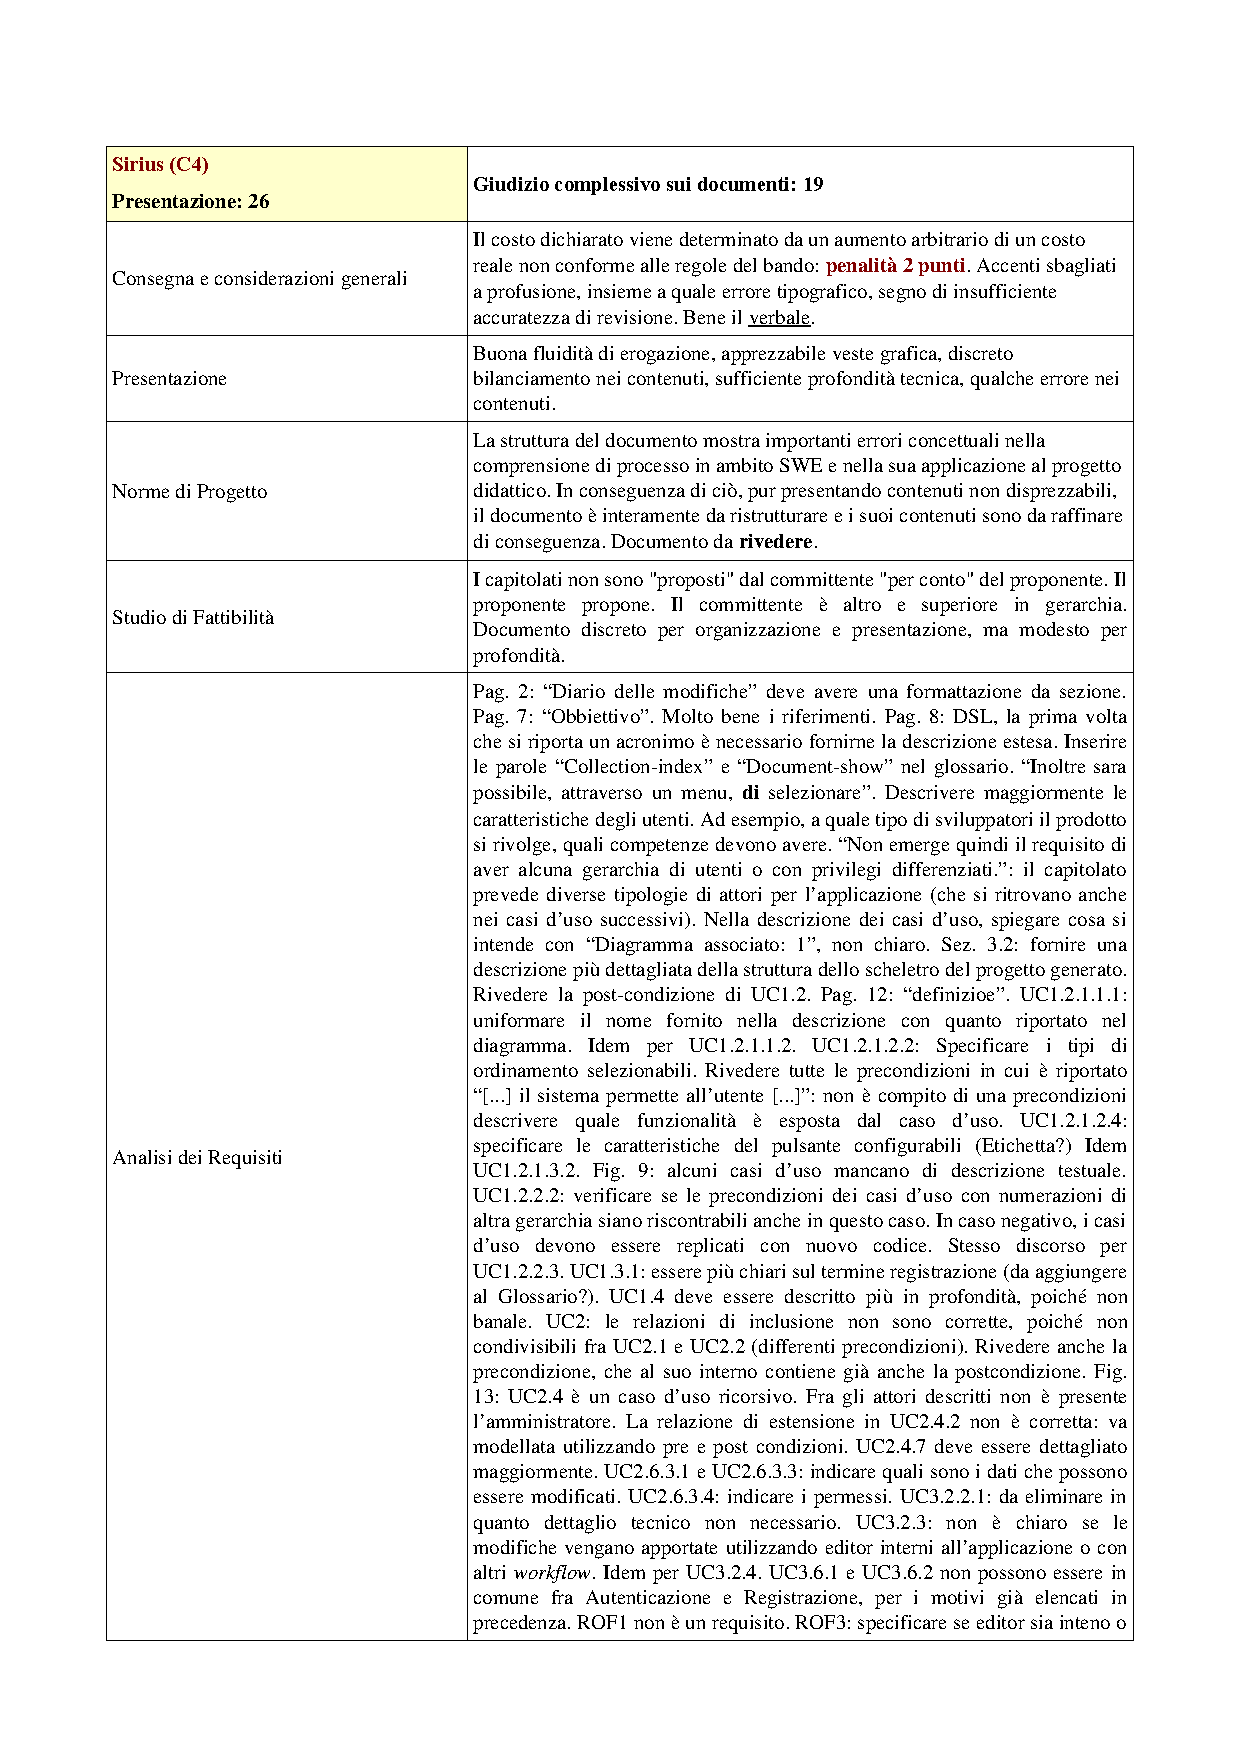
\includegraphics[scale=0.001]{img/Sirius.png}}
        \end{picture}}
	\rhead{\groupname}
	\chead{}
	\lfoot{\info}
	\cfoot{}
%	\rfoot{\thepage}
	\rfoot{\thepage\ / \pageref{LastPage}}
	\renewcommand{\headrulewidth}{0.3pt}
	\renewcommand{\footrulewidth}{0.3pt}
\linespread{1.2}	% valore interlinea


\fancypagestyle{romano}{
	\lhead{\setlength{\unitlength}{1mm}
        \begin{picture}(0,0)
                \put(5,0){
\includegraphics[scale=0.03]{../modello/img/sirius.png}}
        \end{picture}}
	\chead{}
	\rhead{\groupname}
	\lfoot{\info}
	\cfoot{}
	\rfoot{\thepage}
	\renewcommand{\headrulewidth}{0.3pt}
	\renewcommand{\footrulewidth}{0.3pt}
}



\hypersetup{
    colorlinks=true,linkcolor=[rgb]{0.11,0.55,0.83
    },          % colore link interni
    urlcolor=cyan           %colore link esterni
}
\definecolor{err}{rgb}{0.9,0.1,0.1}
\definecolor{rt}{rgb}{0.1,0.6,0.8}
\definecolor{grey}{rgb}{0.4,0.3,0.4}
\definecolor{mycolor}{rgb}{0.67,1,0.18}

\bibliographystyle{plain_ita}%bibliografia stile italiano

\pagenumbering{Roman}
\setlength\parindent{0pt} % sempre senza indentatura
% fine layout% layout

\begin{document}

% Prima pagina di opgni documento
\begin{titlepage}
 \begin{center}
     
\includegraphics[width=11cm]{../modello/img/sirius}\\
     \vspace{1em}
     {\LARGE \textsc{Sirius}}\\
     \vspace{2em} \hrule \vspace{2em}
     {\Large \textsc{Sequenziatore}}\\
     \vspace{8em}
     {\LARGE \LARGE \LARGE \textbf{\doctitle}}\\
     \vspace{2em}
     {\LARGE \LARGE \LARGE \textbf{Versione \lastversion }}\\
     \vspace{4em}
 \end{center}


\vskip 1.8cm
\begin{center}
\textit{Ingegneria Del Software AA 2013-2014}
\end{center}

\end{titlepage}


% pagina del titolo
\thispagestyle{romano}
\noindent\begin{Large}\textbf{Informazioni documento}\end{Large}\\
\begin{center}
\begin{tabular}{ll}
\hline\\
Titolo documento: & Analisi dei requisiti\\
Data creazione: & 1 Febbraio 2014\\
Versione attuale: & \lastversion\\
Utilizzo: & Esterno\\
Nome file:& \AnalisiDeiRequisiti{}\\
Redazione: & Botter Marco\\
& Giachin Vanni\\
& Marcomin Gabriele\\
Verifica: & Seresin Davide\\
Approvazione: & Quaglio Davide\\
Distribuito da:& Sirius\\
Destinato a: & Prof. Vardanega Tullio\\
			 & Prof. Cardin Riccardo\\
			 & Zucchetti S.p.A.
\end{tabular}
\end{center}
\vskip 1.5cm
%\noindent {\begin{LARGE}\textbf{Sommario}\end{LARGE}}\\
\noindent\begin{Large}\textbf{Sommario}\end{Large}\\

\noindent Risultato dello studio di fattibilità della ditta Sirius per il capitolato C04 Seq\\
\newpage
\pagestyle{romano}
\noindent\begin{Large}\textbf{Diario delle modifiche}\end{Large}\\
\\
%Inserire in testa ogni nuova versione\\
\begin{small}
\begin{tabular}{|c|p{1.8cm}|p{2.8cm}|p{2.8cm}|p{3.5cm}|}
\hline
Versione & Data & Autore & Ruolo & Descrizione \\
\hline
\hline
1.0.0 & 2014-03-05 & 
\textit{Quaglio Davide} &
\textit{Responsabile} &  Approvazione del documento\\
\hline
0.1.0 & 2014-02-13 & 
\textit{Botter Marco} &
\textit{Verificatore} &  Verifica del documento\\
\hline
0.0.2 & 2014-02-11 & 
\textit{Seresin Davide} &
\textit{Analista} &  Aggiunte e modifiche\\
\hline
0.0.1 & 2014-02-09 & 
\textit{Santangelo Davide} &
\textit{Analista} &  Creato lo scheletro del documento\\
\hline
\end{tabular}\\
\end{small}


\newpage
\pagestyle{romano}

\tableofcontents %sommario
\pagestyle{romano}



\newpage
\pagestyle{plain}

\pagenumbering{arabic}%numeri di pagina  arabi

\section{Introduzione}

\subsection{Scopo del documento}
Il documento definisce le norme, convenzioni e formalismi  che ciascun membro del gruppo \gruppo{} deve adottare durante l'intera produzione del software \progetto{}.
In particolare tali norme regolamentano i seguenti aspetti:

\begin{itemize}
\item Organizzazione tra i membri del gruppo;
\item Stili e convenzioni nella redazione dei documenti;
\item Metodi operativi e convenzioni nelle fasi di progetto;
\item Ambiente di lavoro.
\end{itemize}

\subsection{Glossario}
Al fine di facilitare la comprensione dei documenti, i termini tecnici, di dominio e gli acronimi, sono definiti in dettaglio nel documento GLOSSARIO.\\
Tali termini sono contrassegnati dal simbolo \ped{$\vert$G$\vert$} che li segue.
\section{Descrizione generale}
\subsection{Prospettive del prodotto}
Il prodotto si pone,in primo luogo, di realizzare dei processi definiti da una serie
di passi che devono essere eseguiti in sequenza, sia con l' obbligo di terminare i passi precedenti
per accedere al passo successivo, sia con la possibilità di eseguire i passi senza
un ordine predefinito.\\
Oltre a questo il sistema dovrà essere capace di gestire l' esecuzione dei vari passi da parte di
utenti dotati di dispositivo mobili di tipo smartphone, ricevendo da questi ultimi la
richiesta di completamento di un passo; esso sarà accompagnato da vari dati come foto, la posizione geografica e il tempo di completamento. Oltre alla esecuzione, il sistema dovrà essere in grado di poter determinare se il passo è stato eseguito con successo o meno, in base ai dati forniti. 
\subsection{Funzionalità del prodotto}
\subsection{Caratteristiche degli utenti}
\subsection{Vincoli generali}

\hypersetup{bookmarksdepth=2}%negli UC per ogni subsubsection i segnalibri vengono definiti a mano
\section{Casi d'uso}

\iffalse  % commento multilinea
\paragraph{UC 1:}
\begin{itemize}
\item \textbf{Attori:} utente autenticato;
\item \textbf{Descrizione:} 
\item \textbf{Precondizione:} 
\item \textbf{Scenario principale:} 
\begin{itemize}
\item 
\end{itemize}
%\item \textbf{Estensioni:} 
%\item \textbf{Inclusioni:} 
%\item \textbf{Scenario alternativo:} 
\item \textbf{Postcondizione:}
\end{itemize}
\fi

\subsection{Ambito utente}

\subsubsection{UCU 0: Caso base utente generico}

\begin{itemize}
\item \textbf{Attori:} utente;
\item \textbf{Descrizione:} l'utente accede alla pagina principale e, per poter accedere alle principali funzionalità, deve autenticarsi.
L'utente non autenticato può registrarsi oppure effettuare il login se è già registrato diventando utente autenticato.
\item \textbf{Precondizione:} il sistema è operativo e l'utente ha iniziato ad interfacciarvisi;
\item \textbf{Scenario principale:}
\begin{itemize}
\item l'utente può effettuare la registrazione;
\item l'utente può effettuare il login e diventare autenticato;
\end{itemize}
%\item \textbf{Scenario alternativo:}
%\item \textbf{Inclusioni:}
\item \textbf{Postcondizione:} il sistema ha eseguito le operazioni desiderate dall'utente.
\end{itemize}

\paragraph{UCU 1: Registrazione}
\begin{itemize}
	\item \textbf{Attori:} utente;
	\item \textbf{Descrizione:} l'utente può registrarsi inserendo i dati richiesti dal sistema;
	\item \textbf{Precondizione:} il sistema é operativo e l'utente ha richiesto la registrazione;
	\item \textbf{Scenario principale:}
	\begin{itemize}
		\item l'utente inserisce lo username scelto;
		\item l'utente inserisce la password scelta;
		\item l'utente inserisce il proprio nome;
		\item l'utente inserisce il proprio cognome;
		\item l'utente inserisce la propria data di nascita;
		%\item l'utente inserisce un proprio numero di telefono.
		\item l'utente inserisce la propria email.
	\end{itemize}
	\item \textbf{Scenario alternativo:}
	\begin{itemize}
		\item un altro utente possiede lo stesso username scelto dall'utente che viene avvisato dell'errore e può scegliere un username diverso;
	\end{itemize}
	\item \textbf{Postcondizione:} il sistema ha salvato i dati immessi dall'utente che ora può autenticarsi.
\end{itemize}

\subparagraph{UCU 1.1: Inserimento username per registrazione}
\begin{itemize}
	\item \textbf{Attori:} utente;
	\item \textbf{Descrizione:} l'utente può inserire il proprio username;
	\item \textbf{Precondizione:} l'utente ha richiesto la registrazione e vuole inserire lo username scelto;
	\item \textbf{Postcondizione:} lo username è stato inserito e il sistema prosegue con la registrazione.
\end{itemize}

\subparagraph{UCU 1.2: Inserimento password per registrazione}
\begin{itemize}
	\item \textbf{Attori:} utente;
	\item \textbf{Descrizione:} l'utente può inserire la propria password;
	\item \textbf{Precondizione:} l'utente ha richiesto la registrazione e vuole inserire la password scelta;
	\item \textbf{Postcondizione:} la password è stata inserita e il sistema prosegue con la registrazione.
\end{itemize}

\subparagraph{UCU 1.3: Inserimento nome per registrazione}
\begin{itemize}
	\item \textbf{Attori:} utente;
	\item \textbf{Descrizione:} l'utente può inserire il proprio nome;
	\item \textbf{Precondizione:} l'utente ha richiesto la registrazione e vuole inserire il proprio nome;
	\item \textbf{Postcondizione:} il nome è stato inserito e il sistema prosegue con la registrazione.
\end{itemize}

\subparagraph{UCU 1.4: Inserimento cognome per registrazione}
\begin{itemize}
	\item \textbf{Attori:} utente.
	\item \textbf{Descrizione:} l'utente può inserire il proprio cognome;
	\item \textbf{Precondizione:} l'utente ha richiesto la registrazione e vuole inserire il proprio cognome;
	\item \textbf{Scenario principale:}
	\item \textbf{Postcondizione:} il cognome è stato inserito e il sistema prosegue con la registrazione.
\end{itemize}

\subparagraph{UCU 1.5: Inserimento data di nascita per registrazione}
\begin{itemize}
	\item \textbf{Attori:} utente;
	\item \textbf{Descrizione:} l'utente può inserire la propria data di nascita;
	\item \textbf{Precondizione:} l'utente ha richiesto la registrazione e vuole inserire la propria data di nascita;
	\item \textbf{Postcondizione:} la data di nascita è stata inserita e il sistema prosegue con la registrazione.
\end{itemize}

\iffalse % ha senso modificare l'username che dovrebbe essere la chiave primaria?
% se si volesse ripristinare queso paragrafo si dovrà anche aggiornare i numeri degli UC.
\subparagraph{UCU 1.6: Inserimento numero di telefono per registrazione}
\begin{itemize}
	\item \textbf{Attori:} utente;
	\item \textbf{Descrizione:} l'utente può inserire il proprio numero di telefono;
	\item \textbf{Precondizione:} l'utente ha richiesto la registrazione e vuole inserire il proprio numero di telefono;
	\item \textbf{Postcondizione:} il numero di telefono è stato inserito e il sistema prosegue con la registrazione utente.
\end{itemize}
\fi

\subparagraph{UCU 1.6: Inserimento email per registrazione}
\begin{itemize}
	\item \textbf{Attori:} utente;
	\item \textbf{Descrizione:} l'utente può inserire una sua email;
	\item \textbf{Precondizione:} l'utente ha richiesto la registrazione e vuole inserire la propria email;
\item \textbf{Postcondizione:} l'email è stata inserita e il sistema prosegue con la registrazione utente.
\end{itemize}

\paragraph{UCU 2: Login}
\begin{itemize}
\item \textbf{Attori:} utente.
\item \textbf{Descrizione:} l'utente può inserire i propri dati d'accesso, ossia lo username e la propria password. Se lo username appartiene all'insieme degli utenti del sistema e la relativa password è corretta, allora l'utente viene autenticato;
\item \textbf{Precondizione:} il sistema è operativo e l'utente non autenticato vuole effettuare il login;
\item \textbf{Scenario principale:}
\begin{itemize}
\item l'utente inserisce il proprio username;
\item l'utente inserisce la propria password.
\end{itemize}
\item \textbf{Scenario alternativo:}
\begin{itemize}
\item le credenziali non risultano essere corrette, viene dunque segnalato l'errore all'utente che può reinserire i dati.
\end{itemize}
\item \textbf{Postcondizione:} l'utente diventa autenticato e il sistema è pronto per consentire la gestione dei processi e dell'account.
\end{itemize}

\subparagraph{UC 2.1: Inserimento username per login}
\begin{itemize}
\item \textbf{Attori:} utente;
\item \textbf{Descrizione:} l'utente può inserire il proprio username;
\item \textbf{Precondizione:} l'utente ha richiesto il login e vuole inserire la propria data di nascita;
\item \textbf{Postcondizione:} lo username è stato inserito e il sistema prosegue con la procedura di autenticazione utente.
\end{itemize}

\subparagraph{UC 2.2: Inserimento password per login}
\begin{itemize}
\item \textbf{Attori:} utente;
\item \textbf{Descrizione:} l'utente può inserire la propria password;
\item \textbf{Precondizione:} l'utente ha richiesto il login e vuole inserire la propria password per il login;
\item \textbf{Postcondizione:} la password è stata inserita e il sistema prosegue con la procedura di autenticazione utente.
\end{itemize}

\subsubsection{UCL 0: Caso base utente autenticato}

\begin{itemize}
\item \textbf{Attori:} utente autenticato;
\item \textbf{Descrizione:} l'utente accede alla pagina principale e, per poter accedere alle principali funzionalità, deve autenticarsi.
L'utente autenticato può gestire il proprio account, gestire un insieme di processi ed effettuare il logout, ritornando allo stato di utente non autenticato;
\item \textbf{Precondizione:} il sistema è operativo, l'utente autenticato ha iniziato ad interfacciarvisi;
\item \textbf{Scenario principale:}
\begin{itemize}
\item l'utente autenticato può gestire il proprio account;
\item l'utente autenticato può gestire i processi disponibili;
\item l'utente autenticato può effettuare il logout diventando utente generico.
\end{itemize}
%\item \textbf{Scenario alternativo:}
%\item \textbf{Inclusioni:}
\item \textbf{Postcondizione:} il sistema ha eseguito le operazioni desiderate dall'utente, salvando eventuali modifiche effettuate all'account e ai processi gestiti.
\end{itemize}

\paragraph{UCL 1: Gestione dell'account} %opt
\begin{itemize}
	\item \textbf{Attori:} utente autenticato;
	\item \textbf{Descrizione:} l'utente visualizza i dati salvati nel sistema relativi al suo account e può modificarli;
	\item \textbf{Precondizione:} l'utente autenticato vuole gestire i propri dati;
	\item \textbf{Scenario principale:}
	\begin{itemize}
		\item l'utente può visualizzare i propri dati;
		\item l'utente può modificare i propri dati.
	\end{itemize}
	\item \textbf{Postcondizione:} il sistema ha eseguito e salvato le operazioni effettuate dall'utente sui dati del suo account.
\end{itemize}

\subparagraph{UCL 1.1: Visualizzazione dei dati dell'utente}
\begin{itemize}
	\item \textbf{Attori:} utente autenticato.
	\item \textbf{Descrizione:} l'utente può visualizzare i dati salvati nel sistema relativi al suo account;
	\item \textbf{Precondizione:} l'utente vuole gestire i suoi dati;
	\item \textbf{Scenario principale:}
	\begin{itemize}
		\item l'utente visualizza il suo username;
		\item l'utente visualizza il suo nome;
		\item l'utente visualizza il suo cognome;
		\item l'utente visualizza la sua data di nascita;
		\item l'utente visualizza la sua email.
		%\item l'utente visualizza il suo numero di telefono.
	\end{itemize}
	\item \textbf{Postcondizione:} il sistema ha visualizzato i dati dell'account dell'utente.
\end{itemize}

\subparagraph{UCL 1.1.1: Visualizzazione username}
\begin{itemize}
	\item \textbf{Attori:} utente autenticato.
	\item \textbf{Descrizione:} l'utente può visualizzare il suo username;
	\item \textbf{Precondizione:} l'utente vuole visualizzare i suoi dati;
\item \textbf{Postcondizione:} il sistema ha visualizzato lo username dell'utente.
\end{itemize}

\subparagraph{UCL 1.1.2: Visualizzazione nome}
\begin{itemize}
	\item \textbf{Attori:} utente autenticato;
	\item \textbf{Descrizione:} l'utente può visualizzare il suo nome;
	\item \textbf{Precondizione:} l'utente vuole visualizzare i suoi dati;
	\item \textbf{Postcondizione:} il sistema ha visualizzato il nome dell'utente.
\end{itemize}

\subparagraph{UCL 1.1.3: Visualizzazione cognome}
\begin{itemize}
	\item \textbf{Attori:} utente autenticato;
	\item \textbf{Descrizione:} l'utente può visualizzare il suo cognome;
	\item \textbf{Precondizione:} l'utente vuole visualizzare i suoi dati;
	\item \textbf{Postcondizione:} il sistema ha visualizzato il cognome dell'utente.
\end{itemize}

\subparagraph{UCL 1.1.4: Visualizzazione data di nascita}
\begin{itemize}
	\item \textbf{Attori:} utente autenticato;
	\item \textbf{Descrizione:} l'utente può visualizzare la sua data di nascita;
	\item \textbf{Precondizione:} l'utente vuole visualizzare i suoi dati;
	\item \textbf{Postcondizione:} il sistema ha visualizzato la data di nascita dell'utente.
\end{itemize}

\iffalse % ha senso il campo dati telefono?
% se si volesse ripristinare queso paragrafo si dovrà anche aggiornare i numeri degli UC.
\subparagraph{UCL 1.1.5: Visualizzazione numero di telefono}
\begin{itemize}
	\item \textbf{Attori:} utente autenticato;
	\item \textbf{Descrizione:} l'utente può visualizzare il numero di telefono salvato nel sistema;
	\item \textbf{Precondizione:} l'utente vuole visualizzare i suoi dati;
	\item \textbf{Scenario principale:}
	\begin{itemize}
	 \item l'utente visualizza il proprio numero di telefono.
	\end{itemize}
	\item \textbf{Postcondizione:} il sistema ha visualizzato il numero di telefono dell'utente.
\end{itemize}
\fi

\subparagraph{UCL 1.1.5: Visualizzazione email}
\begin{itemize}
	\item \textbf{Attori:} utente autenticato;
	\item \textbf{Descrizione:} l'utente può visualizzare la sua email salvata nel sistema;
	\item \textbf{Precondizione:} l'utente vuole visualizzare i suoi dati;
	\item \textbf{Scenario principale:}
	\begin{itemize}
	 \item l'utente visualizza la propria email.
	\end{itemize}
	\item \textbf{Postcondizione:} il sistema ha visualizzato l'email dell'utente.
\end{itemize}

 
\subparagraph{UCL 1.2: Modifica dati utente} %opt
\begin{itemize}
	\item \textbf{Attori:} utente autenticato.
	\item \textbf{Descrizione:} l'utente vuole modificare i dati salvati nel sistema relativi al suo account;
	\item \textbf{Precondizione:} l'utente vuole gestire i suoi dati;
	\item \textbf{Scenario principale:}
	\begin{itemize}
		%\item l'utente può modificare il suo username;
		\item l'utente può modificare la sua password;
		%\item l'utente può modificare il suo nome;
		%\item l'utente può modificare il suo cognome;
		%\item l'utente può modificare il suo numero di telefono;
		\item l'utente può modificare la sua email.
	\end{itemize}
\item \textbf{Postcondizione:} il sistema ha salvato le modiche dei dati dell'utente.
\end{itemize}

\iffalse % ha senso modificare l'username che dovrebbe essere la chiave primaria?
% se si volesse ripristinare queso paragrafo, si dovrà anche correggerlo e aggiornari i numeri degli UC.
\subparagraph{UCL 1.2.1: Modifica username}
\begin{itemize}
	\item \textbf{Attori:} utente autenticato.
	\item \textbf{Descrizione:} l'utente inserisce il proprio username, e se lo username risulta non è gia stato utilizzato da un altro utente, allora la modifica verrà salvata dal sistema
	\item \textbf{Precondizione:} l'utente vuole modicare il suo username.
	\item \textbf{Scenario principale:}
	\begin{itemize}
		\item l'utente inserisce il nuovo username scelto.
	\end{itemize}
	\item \textbf{Scenario alternativo:}
	\begin{itemize}
		\item il nuovo username è gia presente nel sistema, ne viene data comunicazione dell'errore e della possibilità di reinserire un username diverso.
	\end{itemize}
\item \textbf{Postcondizione:} il cambiamento di username viene salvato dal sistema.
\end{itemize}
\fi

\subparagraph{UCL 1.2.1: Modifica password}
\begin{itemize}
	\item \textbf{Attori:}  utente autenticato;
	\item \textbf{Descrizione:} per modificare la password d'accesso, l'utente deve inserire la password corrente e la nuova password scelta. Se i dati immessi risultano corretti vengono salvati dal sistema, altrimenti l'errore viene segnalato all'utente che dovrà correggerli;
	\item \textbf{Precondizione:} l'utente vuole modificare la sua password;
	\item \textbf{Scenario principale:}
	\begin{itemize}
		\item l'utente inserisce la password attualmente salvata;
		\item l'utente inserisce la nuova password scelta.
	\end{itemize}
	\item \textbf{Scenario alternativo:}
	\begin{itemize}
		\item la password corrente immessa non è corretta, l'errore viene segnalato all'utente che può reinserire la password.
	\end{itemize}
	\item \textbf{Postcondizione:} il sistema ha salvato la nuova password scelta dall'utente.
\end{itemize}

\subparagraph{UCL 1.2.1.1: Inserimento password corrente}
\begin{itemize}
	\item \textbf{Attori:} utente autenticato;
	\item \textbf{Descrizione:} l'utente può inserire la password corrente;
	\item \textbf{Precondizione:} l'utente vuole modificare la sua password;
	\item \textbf{Postcondizione:} la password corrente è stata inserita e il sistema prosegue con la procedura di modifica della password.
\end{itemize}

\subparagraph{UCL 1.2.1.2 Inserimento nuova password}
\begin{itemize}
	\item \textbf{Attori: } utente autenticato;
	\item \textbf{Descrizione:} l'utente può inserire la nuova password scelta;
	\item \textbf{Precondizione:} l'utente vuole modificare la sua password;
	\item \textbf{Postcondizione:} la nuova password è stata inserita e il sistema prosegue con la procedura di modifica della password.
\end{itemize}

\iffalse % ha senso modificare nome e cognome?
% se si volesse ripristinare quesi paragrafi, si dovrà anche correggerli e aggiornari i numeri degli UC.
\subparagraph{UCL 1.2.2.3 Modifica nome}
\begin{itemize}
	\item \textbf{Attori: } utente autenticato.
	\item \textbf{Descrizione: } l'utente inserisce il nuovo nome, il sistema procede con il salvataggio delle modifiche
	\item \textbf{Precondizione: } l'utente vuole modicare il suo nome salvato nel sistema.
	\item \textbf{Postcondizione:} la modifica del nome viene salvato dal sistema.
\end{itemize}

\subparagraph{UCL 1.2.2.4  Modifica cognome}
\begin{itemize}
	\item \textbf{Attori: }  utente autenticato.
	\item \textbf{Descrizione: } l'utente inserisce il nuovo cognome, il sistema procede con il salvataggio del dato.
	\item \textbf{Precondizione: } l'utente vuole cambiare il suo cognome salvato nel sistema.
	\item \textbf{Postcondizione:} il nuovo cognome viene salvato dal sistema.
\end{itemize}
\fi

\iffalse
\subparagraph{UCL 1.2.2  Modifica numero di telefono}
\begin{itemize}
\item \textbf{Attori: } utente autenticato;
\item \textbf{Descrizione: } l'utente inserisce il nuovo numero di telefono e il sistema procede con la modifica;
\item \textbf{Precondizione: } l'utente vuole modificare il numero di telefono salvato;
\item \textbf{Postcondizione:} il sistema ha salvato il nuovo di numero di telefono scelto dall'utente.
\end{itemize}
\fi

\subparagraph{UCL 1.2.2  Modifica email}
\begin{itemize}
\item \textbf{Attori:} utente autenticato;
\item \textbf{Descrizione:} l'utente inserisce una nuova email per modificare l'email salvata nel sistema;
\item \textbf{Precondizione:} l'utente vuole modificare l'email salvata nel sistema;
\item \textbf{Postcondizione:} il sistema ha salvato la nuova email scelta dall'utente.
\end{itemize}

\paragraph{UCL 2: Gestione dei processi}
\begin{itemize}
\item \textbf{Attori:} utente autenticato;
\item \textbf{Descrizione:} l'utente può scegliere un processo per gestirlo.
Se l'utente non è iscritto al processo può iscrivervisi, altrimenti può eseguirlo o disiscriversi da esso.
Scegliendo un processo l'utente può inoltre visualizzarne le informazioni;
\item \textbf{Precondizione:} l'utente autenticato vuole gestire i processi a cui può partecipare;
\item \textbf{Scenario principale:}
\begin{itemize}
\item l'utente può scegliere un processo;
\item l'utente può visualizzare la descrizione di un processo;
\item l'utente può iscriversi a un processo a cui non è già iscritto;
\item l'utente può eseguire un processo a cui è iscritto;
\item l'utente può disiscriversi da un processo a cui è iscritto.
\end{itemize}
%\item \textbf{Scenario alternativo:}
%\item \textbf{Estensioni:}
\item \textbf{Postcondizione:} il sistema ha eseguito e salvato le operazioni desiderate dall'utente sui processi selezionati.
\end{itemize}

\subparagraph{UCL 2.1: Scelta di un processo}
\begin{itemize}
\item \textbf{Attori:} utente autenticato;
\item \textbf{Descrizione:} l'utente può selezionare un processo da una lista selezionata o da i risultati di una ricerca;
\item \textbf{Precondizione:} l'utente autenticato vuole gestire un processo tra quelli a cui può partecipare;
\item \textbf{Flusso principale degli eventi:}
\begin{enumerate}
\item l'utente può aprire una lista di processi;
\item l'utente può selezionare un processo.
\end{enumerate}
\item \textbf{Estensioni:} l'utente può effettuare la ricerca di un processo;
%\item \textbf{Inclusioni:}
\item \textbf{Postcondizione:} il sistema è pronto per la gestione del processo scelto.
%\item \textbf{Scenario alternativo:}
\end{itemize}

\subparagraph{UCL 2.1.1: Apertura di una lista di processi}
\begin{itemize}
\item \textbf{Attori:} utente autenticato;
\item \textbf{Descrizione:} l'utente può scegliere e aprire una lista di processi;
\item \textbf{Precondizione:} l'utente vuole scegliere un processo tra quelli a cui può partecipare;
\item \textbf{Scenario principale:}
\begin{itemize}
\item l'utente può aprire la lista dei processi a cui è iscritto;
\item l'utente può aprire la lista dei processi a cui non è iscritto;
\end{itemize}
%\item \textbf{Scenario alternativo:}
\item \textbf{Inclusioni:}
\begin{itemize}
\item i processi in attesa di terminazione vengono segnalati all'utente;
\item i nuovi processi vengono segnalati all'utente;
\end{itemize}
%\item \textbf{Estensioni:}
\item \textbf{Postcondizione:} il sistema ha visualizzato la lista dei processi scelta dall'utente.
\end{itemize}

\subparagraph{UCL 2.1.1.1: Apertura lista dei processi in esecuzione}
\begin{itemize}
\item \textbf{Attori:} utente autenticato;
\item \textbf{Descrizione:} l'utente può aprire e visualizzare la lista dei processi in esecuzione, cioè quelli a cui è già iscritto. 
\item \textbf{Precondizione:} l'utente vuole aprire la lista dei processi a cui è iscritto;
%\item \textbf{Scenario alternativo:}
%\item \textbf{Estensioni:}
\item \textbf{Postcondizione:} il sistema ha visualizzato la lista dei processi a cui l'utente è iscritto.
\end{itemize}

\subparagraph{UCL 2.1.1.2: Apertura lista dei processi disponibili}
\begin{itemize}
\item \textbf{Attori:} utente autenticato;
\item \textbf{Descrizione:} l'utente può aprire e visualizzare la lista dei processi disponibili, cioè quelli a cui non è iscritto;
\item \textbf{Precondizione:} l'utente vuole aprire la lista dei processi disponibili;
%\item \textbf{Scenario alternativo:}
%\item \textbf{Estensioni:}
\item \textbf{Postcondizione:} il sistema ha visualizzato la lista dei processi a cui l'utente non è iscritto.
\end{itemize}

\subparagraph{UCL 2.1.1.3: Segnalazione dei processi terminabili}
\begin{itemize}
\item \textbf{Attori:} utente autenticato;
\item \textbf{Descrizione:} i processi terminati presenti nella lista dei processi in esecuzione, vengono segnalati all'utente. 
\item \textbf{Precondizione:} l'ha sta visualizzando la lista dei processi in esecuzione;
%\item \textbf{Scenario alternativo:}
%\item \textbf{Inclusioni:}
%\item \textbf{Estensioni:}
\item \textbf{Postcondizione:} il sistema ha evidenziato i processi terminabili dall'utente.
\end{itemize}

\subparagraph{UCL 2.1.1.4: Segnalazione dei nuovi processi}
\begin{itemize}
\item \textbf{Attori:} utente autenticato;
\item \textbf{Descrizione:} i processi mai aperti dall'utente, vengono segnalati come nuovi. 
\item \textbf{Precondizione:} l'ha sta visualizzando la lista dei processi disponibili;
%\item \textbf{Scenario alternativo:}
%\item \textbf{Inclusioni:}
%\item \textbf{Estensioni:}
\item \textbf{Postcondizione:} il sistema ha evidenziato i nuovi processi disponibili all'utente.
\end{itemize}

\subparagraph{UCL 2.1.2: Selezione di un processo}
\begin{itemize}
\item \textbf{Attori:} utente autenticato;
\item \textbf{Descrizione:} l'utente può selezionare un processo dalla lista dei processi precedentemente aperta;
\item \textbf{Precondizione:} l'utente sta visualizzando una lista di uno o più processi;
%\item \textbf{Scenario alternativo:}
%\item \textbf{Inclusioni:}
%\item \textbf{Estensioni:}
\item \textbf{Postcondizione:} il sistema è pronto per la gestione del processo scelto.
\end{itemize}

\subparagraph{UCL 2.1.3: Ricerca di un processo}
\begin{itemize}
\item \textbf{Attori:} utente autenticato;
\item \textbf{Descrizione:} l'utente può ricercare un insieme di processi tra tutti quelli a cui può partecipare;
\item \textbf{Precondizione:} l'utente vuole cercare un processo tra quelli a cui può partecipare;
%\item \textbf{Inclusioni:}
%\item \textbf{Estensioni:}
\item \textbf{Postcondizione:} il sistema ha visualizzato la lista dei processi che soddisfano i criteri di ricerca.
\end{itemize}

\subparagraph{UCL 2.2: Visualizzazione della descrizione di un processo}
\begin{itemize}
\item \textbf{Attori:} utente autenticato;
\item \textbf{Descrizione:} nella pagina di gestione di un processo selezionato l'utente può visualizzarne la descrizione, che spiega lo scopo del processo;
\item \textbf{Precondizione:} il sistema ha aperto la pagina di gestione di un processo;
%\item \textbf{Estensioni:} 
%\item \textbf{Inclusioni:} 
%\item \textbf{Scenario alternativo:} 
\item \textbf{Postcondizione:}
\end{itemize} il sistema ha visualizzato la descrizione del processo gestito.

\subparagraph{UCL 2.3: Iscrizione ad un processo}
\begin{itemize}
\item \textbf{Attori:} utente autenticato;
\item \textbf{Descrizione:} l'utente può iscriversi ad un processo a cui non è ancora iscritto;
\item \textbf{Precondizione:} il sistema ha aperto la pagina di gestione di un processo e l'utente non è iscritto ad esso;
%\item \textbf{Scenario alternativo:}
%\item \textbf{Inclusioni:}
%\item \textbf{Estensioni:}
\item \textbf{Postcondizione:} l'utente è iscritto al processo gestito e il sistema è pronto per la sua esecuzione.
\end{itemize}

\subparagraph{UCL 2.4: Esecuzione di un processo}
\begin{itemize}
\item \textbf{Attori:} utente autenticato;
\item \textbf{Descrizione:} l'utente può visualizzare lo stato di avanzamento e i criteri di terminazione del processo e procedere all'esecuzione di un passo;
\item \textbf{Precondizione:} il sistema ha aperto la pagina di gestione di un processo e l'utente è iscritto ad esso;
\item \textbf{Flusso principale degli eventi:}
\begin{enumerate}
\item l'utente può visualizzazione i criteri di terminazione del processo;
\item l'utente può visualizzare lo stato dell'esecuzione del processo;
\item l'utente può visualizzare la lista dei passi in corso;
\item l'utente può eseguire un passo del processo.
\item l'utente può concludere l'esecuzione di un processo;
\end{enumerate} 
%\item \textbf{Inclusioni:}
%\item \textbf{Estensioni:}
\item \textbf{Postcondizione:} il sistema ha eseguito e salvato le operazioni effettuate dall'utente sul processo gestito.
\end{itemize}

\subparagraph{UCL 2.4.1: Visualizzazione dei criteri di terminazione di un processo}
\begin{itemize}
\item \textbf{Attori:} utente autenticato;
\item \textbf{Descrizione:} l'utente può visualizzare i criteri di terminazione del processo selezionato. Questi criteri sono il completamento del processo da parte di un certo numero di utenti ed eventualmente una precisa data di scadenza;
\item \textbf{Precondizione:} il sistema ha aperto la pagina di gestione di un processo non terminato e l'utente è iscritto ad esso;
\item \textbf{Scenario principale:}
\begin{itemize}
\item l'utente può visualizzare il numero di completamenti che causano la terminazione del processo;
\item l'utente può visualizzare l'eventuale data di scadenza del processo.
\end{itemize}
%\item \textbf{Estensioni:}
%\item \textbf{Inclusioni:}
%\item \textbf{Scenario alternativo:} 
\item \textbf{Postcondizione:} il sistema ha visualizzato i criteri di terminazione del processo gestito.
\end{itemize}

\subparagraph{UCL 2.4.1.1: Visualizzazione massimo numero possibile di completamenti del processo}
\begin{itemize}
\item \textbf{Attori:} utente autenticato;
\item \textbf{Descrizione:} l'utente può visualizzare il numero di completamenti del processo, necessario e sufficiente a causarne la terminazione;
\item \textbf{Precondizione:} il sistema ha aperto la pagina di gestione di un processo non terminato e l'utente è iscritto ad esso;
%\item \textbf{Estensioni:}
%\item \textbf{Inclusioni:}
%\item \textbf{Scenario alternativo:} 
\item \textbf{Postcondizione:} il sistema ha visualizzato il numero di completamenti che causano la terminazione del processo.
\end{itemize}

\subparagraph{UCL 2.4.1.2: Visualizzazione data di scadenza del processo}
\begin{itemize}
\item \textbf{Attori:} utente autenticato;
\item \textbf{Descrizione:} l'utente può visualizzare l'eventuale data di scadenza del processo;
\item \textbf{Precondizione:} il sistema ha aperto la pagina di gestione di un processo  non terminato e con una data di scadenza, e l'utente è iscritto ad esso;
%\item \textbf{Estensioni:}
%\item \textbf{Inclusioni:}
%\item \textbf{Scenario alternativo:} 
\item \textbf{Postcondizione:} il sistema ha visualizzato la data di scadenza del processo.
\end{itemize}

\subparagraph{UCL 2.4.2: Visualizzazione dello stato del processo}
\begin{itemize}
\item \textbf{Attori:} utente autenticato;
\item \textbf{Descrizione:} l'utente può visualizzare informazioni sullo stato di avanzamento del processo. In particolare può visualizzare il numero di passi completati, il totale dei passi, il numero di utenti che hanno completato il processo e il numero di utenti iscritti al processo;
\item \textbf{Precondizione:} il sistema ha aperto la pagina di gestione di un processo e l'utente è iscritto ad esso;
\begin{itemize}
\item l'utente visualizza il numero di passi che ha completato;
\item l'utente visualizza il numero totale di passi del processo;
\item l'utente visualizza il numero di utenti che hanno completato il processo;
\item l'utente visualizza il numero di utenti iscritti al processo.
\end{itemize}
%\item \textbf{Estensioni:}
%\item \textbf{Inclusioni:}
%\item \textbf{Scenario alternativo:} 
\item \textbf{Postcondizione:} il sistema ha visualizzato le informazioni sullo stato di avanzamento del processo.
\end{itemize}

\subparagraph{UCL 2.4.2.1: visualizzazione numero di passi completati}
\begin{itemize}
\item \textbf{Attori:} utente autenticato;
\item \textbf{Descrizione:} l'utente può visualizzare il numero di passi completati del processo;
\item \textbf{Precondizione:} il sistema ha aperto la pagina di gestione di un processo e l'utente è iscritto ad esso;
%\item \textbf{Scenario alternativo:}
%\item \textbf{Inclusioni:}
%\item \textbf{Estensioni:}
\item \textbf{Postcondizione:} il sistema ha visualizzato il numero di passi del processo gestito completati dall'utente.
\end{itemize}

\subparagraph{UCL 2.4.2.2: visualizzazione numero totale dei passi}
\begin{itemize}
\item \textbf{Attori:} utente autenticato;
\item \textbf{Descrizione:} l'utente può visualizzare il numero di passi del processo;
\item \textbf{Precondizione:} il sistema ha aperto la pagina di gestione di un processo e l'utente è iscritto ad esso;
%\item \textbf{Scenario alternativo:}
%\item \textbf{Inclusioni:}
%\item \textbf{Estensioni:}
\item \textbf{Postcondizione:} il sistema ha visualizzato il numero dei passi del processo gestito.
\end{itemize}

\subparagraph{UCL 2.4.2.3: visualizzazione numero di completamenti del processo}
\begin{itemize}
\item \textbf{Attori:} utente autenticato;
\item \textbf{Descrizione:} l'utente può visualizzare il numero di utenti che hanno completato il processo gestito;
\item \textbf{Precondizione:} il sistema ha aperto la pagina di gestione di un processo e l'utente è iscritto ad esso;
%\item \textbf{Scenario alternativo:}
%\item \textbf{Inclusioni:}
%\item \textbf{Estensioni:}
\item \textbf{Postcondizione:} il sistema ha visualizzato di utenti che hanno completato il processo gestito.
\end{itemize}

\subparagraph{UCL 2.4.2.4: visualizzazione numero di iscritti al processo}
\begin{itemize}
\item \textbf{Attori:} utente autenticato;
\item \textbf{Descrizione:} l'utente può visualizzare il numero di utenti iscritti al processo;
\item \textbf{Precondizione:} il sistema ha aperto la pagina di gestione di un processo e l'utente è iscritto ad esso;
%\item \textbf{Scenario alternativo:}
%\item \textbf{Inclusioni:}
%\item \textbf{Estensioni:}
\item \textbf{Postcondizione:} il sistema ha visualizzato il numero di utenti iscritti al processo gestito.
\end{itemize}

\subparagraph{UCL 2.4.3: visualizzazione della lista dei passi in corso}
\begin{itemize}
\item \textbf{Attori:} utente autenticato;
\item \textbf{Descrizione:} l'utente può visualizzare la lista passi non ancora conclusi, immediatamente successivi agli ultimi passi superati;
\item \textbf{Precondizione:} il sistema ha aperto la pagina di gestione di un processo non terminato, l'utente è iscritto ad esso e non lo ha concluso;
%\item \textbf{Scenario alternativo:}
%\item \textbf{Inclusioni:}
%\item \textbf{Estensioni:}
\item \textbf{Postcondizione:} il sistema ha visualizzato la lista dei passo in corso ed è pronto per gestirli.
\end{itemize}

\subparagraph{UCL 2.4.4: Esecuzione di un passo}
\begin{itemize}
\item \textbf{Attori:} utente autenticato;
\item \textbf{Descrizione:} l'utente può visualizzare i criteri di terminazione di un passo del processo, inserire i dati richiesti e procedere all'invio dei dati immessi. In seguito all'invio dei dati l'utente riceverà una notifica;
\item \textbf{Precondizione:} l'utente sta visualizzando la lista dei passi in corso e il sistema è pronto alla loro gestione;
\item \textbf{Flusso principale degli eventi:}
\begin{enumerate}
\item l'utente può visualizzare le informazioni sul passo;
\item l'utente può visualizzare i vincoli di un passo;
\item l'utente può inserire i dati richiesti da un passo;
\item l'utente può inviare al sistema i dati richiesti da un passo;
\item l'utente può concludere un passo.
\end{enumerate}
%\item \textbf{Scenario alternativo:}
\item \textbf{Inclusioni:} l'utente dopo aver inviato i dati può visualizzare l'esito dell'esecuzione del passo;
\item \textbf{Estensioni:} l'utente può saltare i passi opzionali;
\item \textbf{Postcondizione:} il sistema ha eseguito e salvato le operazioni effettuate dall'utente sul passo eseguito e ritorna alla gestione del processo.
\end{itemize}

\subparagraph{UCL 2.4.4.1: Visualizzazione delle informazioni di un passo}
\begin{itemize}
\item \textbf{Attori:} utente autenticato;
\item \textbf{Descrizione:} l'utente può visualizzare l'eventuale descrizione del passo e le eventuali descrizioni dei dati richiesti;
\item \textbf{Precondizione:} il sistema è pronto alla gestione dei passi del processo;
%\item \textbf{Scenario alternativo:}
%\item \textbf{Inclusioni:} l'utente dopo aver inviato i dati può visualizzare l'esito dell'esecuzione del passo;
%\item \textbf{Estensioni:} 
\item \textbf{Postcondizione:} il sistema ha visualizzato le informazioni sul passo.
\end{itemize}

\subparagraph{UCL 2.4.4.2: Visualizzazione dei vincoli di un passo}
\begin{itemize}
\item \textbf{Attori:} utente autenticato;
\item \textbf{Descrizione:} l'utente può visualizzare i vincoli sui dati richiesti e sull'approvazione del passo;
\item \textbf{Precondizione:} il sistema è pronto alla gestione dei passi del processo;
\item \textbf{Scenario principale:}
\begin{itemize}
\item l'utente può visualizzare i vincoli sull'approvazione del passo;
\item l'utente può visualizzare i vincoli sulle coordinate;
\item l'utente può visualizzare i vincoli temporali;
\item l'utente può visualizzare i vincoli sui dati numerici.
\end{itemize}
%\item \textbf{Scenario alternativo:}
%\item \textbf{Inclusioni:} l'utente dopo aver inviato i dati può visualizzare l'esito dell'esecuzione del passo;
%\item \textbf{Estensioni:} 
\item \textbf{Postcondizione:} il sistema ha visualizzato i vincoli sui dati da inserire.
\end{itemize}

\subparagraph{UCL 2.4.4.2.1: Visualizzazione dei vincoli sull'approvazione}
\begin{itemize}
\item \textbf{Attori:} utente autenticato;
\item \textbf{Descrizione:} l'utente può visualizzare se il passo gestito richiede l'approvazione dell'amministratore per essere concluso;
\item \textbf{Precondizione:} il sistema è pronto alla gestione dei passi del processo;
%\item \textbf{Scenario alternativo:}
%\item \textbf{Inclusioni:} l'utente dopo aver inviato i dati può visualizzare l'esito dell'esecuzione del passo;
%\item \textbf{Estensioni:} 
\item \textbf{Postcondizione:} il sistema ha visualizzato i vincoli sull'approvazione del passo gestito.
\end{itemize}

\subparagraph{UCL 2.4.4.2.2: Visualizzazione dei vincoli sulle coordinate}
\begin{itemize}
\item \textbf{Attori:} utente autenticato;
\item \textbf{Descrizione:} l'utente può visualizzare i vincoli sui dati geografici richiesti. Questi vincoli sono espressi tramite l'indicazione di un luogo preciso e di un'eventuale raggio di tolleranza rispetto al luogo indicato;
\item \textbf{Precondizione:} il sistema di gestione del passo gestito richiede l'invio delle coordinate geografiche dell'utente;
%\item \textbf{Scenario alternativo:}
%\item \textbf{Inclusioni:} l'utente dopo aver inviato i dati può visualizzare l'esito dell'esecuzione del passo;
%\item \textbf{Estensioni:} 
\item \textbf{Postcondizione:} il sistema ha visualizzato i vincoli sulle coordinate richieste dal passo gestito.
\end{itemize}

\subparagraph{UCL 2.4.4.2.3: Visualizzazione dei vincoli temporali}
\begin{itemize}
\item \textbf{Attori:} utente autenticato;
\item \textbf{Descrizione:} l'utente può visualizzare gli intervalli temporali in cui l'utente può inviare i dati;
\item \textbf{Precondizione:} il sistema di gestione del passo gestito richiede la data e l'ora dell'invio dei dati;
%\item \textbf{Scenario alternativo:}
%\item \textbf{Inclusioni:} l'utente dopo aver inviato i dati può visualizzare l'esito dell'esecuzione del passo;
%\item \textbf{Estensioni:} 
\item \textbf{Postcondizione:} il sistema ha visualizzato i vincoli sui tempi di invio dei dati.
\end{itemize}

\subparagraph{UCL 2.4.4.2.4: Visualizzazione dei vincoli sui dati numerici}
\begin{itemize}
\item \textbf{Attori:} utente autenticato;
\item \textbf{Descrizione:} l'utente può visualizzare i vincoli sui dati numerici che possono essere il numero di cifre, la possibilità di inserire cifre decimali o meno, e un eventuale limite superiore o inferiore;
\item \textbf{Precondizione:} il sistema di gestione del passo gestito richiede l'inserimento di un valore numerico;
%\item \textbf{Scenario alternativo:}
%\item \textbf{Inclusioni:} l'utente dopo aver inviato i dati può visualizzare l'esito dell'esecuzione del passo;
%\item \textbf{Estensioni:} 
\item \textbf{Postcondizione:} il sistema ha visualizzato i vincoli sui dati numerici richiesti dal passo gestito.
\end{itemize}

\subparagraph{UCL 2.4.4.3: Inserimento dei dati richiesti}
\begin{itemize}
\item \textbf{Attori:} utente autenticato;
\item \textbf{Descrizione:} l'utente può inserire i dati richiesti per l'esecuzione del passo in corso. Può essere richiesto il caricamento di foto, di testo o di dati numerici; 
\item \textbf{Precondizione:} il sistema di gestione del passo richiede l'inserimento di uno o più dati;
\item \textbf{Scenario principale:}
\begin{itemize}
\item l'utente può inserire un'immagine;
\item l'utente può inserire del testo;
\item l'utente può inserire dei dati numerici.
\end{itemize}
%\item \textbf{Scenario alternativo:}
%\item \textbf{Inclusioni:}
%\item \textbf{Estensioni:}
\item \textbf{Postcondizione:} i dati inseriti dall'utente sono pronti per essere inviati al sistema.
\end{itemize}

\subparagraph{UCL 2.4.4.3.1: Inserimento di un'immagine}
\begin{itemize}
\item \textbf{Attori:} utente autenticato;
\item \textbf{Descrizione:} l'utente può inserire un'immagine scattando una foto o caricandola dai propri file;
\item \textbf{Precondizione:} il sistema di gestione del passo richiede l'inserimento di uno o più immagini;
\item \textbf{Scenario principale:}
\begin{itemize}
\item l'utente può inserire un'immagine scattando una foto;
\item l'utente può inserire un'immagine caricandola dai propri file;
\end{itemize}
%\item \textbf{Scenario alternativo:}
%\item \textbf{Inclusioni:}
%\item \textbf{Estensioni:}
\item \textbf{Postcondizione:} l'immagine inserita dall'utente è pronta per essere inviata al sistema.
\end{itemize}

\subparagraph{UCL 2.4.4.3.1.1: Inserimento di una foto scattata}
\begin{itemize}
\item \textbf{Attori:} utente autenticato;
\item \textbf{Descrizione:} l'utente può scattare una foto per inserire l'immagine richiesta dal passo in corso;
\item \textbf{Precondizione:} l'utente vuole scattare una foto per inserire l'immagine richiesta dal passo gestito;
%\item \textbf{Scenario alternativo:}
%\item \textbf{Inclusioni:}
%\item \textbf{Estensioni:}
\item \textbf{Postcondizione:} la foto scattata dall'utente è pronta per essere inviata al sistema.
\end{itemize}

\subparagraph{UCL 2.4.4.3.1.2: Inserimento di un'immagine da file}
\begin{itemize}
\item \textbf{Attori:} utente autenticato;
\item \textbf{Descrizione:} l'utente può caricare un'immagine dai suoi file per soddisfare la richiesta del passo in corso;
\item \textbf{Precondizione:} l'utente vuole scattare una foto per inserire l'immagine richiesta dal passo gestito;
%\item \textbf{Scenario alternativo:}
%\item \textbf{Inclusioni:}
%\item \textbf{Estensioni:}
\item \textbf{Postcondizione:} la foto scattata dall'utente è pronta per essere inviata al sistema.
\end{itemize}

\subparagraph{UCL 2.4.4.3.2: Inserimento di dati testuali}
\begin{itemize}
\item \textbf{Attori:} utente autenticato;
\item \textbf{Descrizione:} l'utente può inserire i dati testuali richiesti dal passo in corso;
\item \textbf{Precondizione:} il sistema di gestione del passo richiede l'inserimento di dati testuali;
%\item \textbf{Scenario alternativo:}
%\item \textbf{Inclusioni:}
%\item \textbf{Estensioni:}
\item \textbf{Postcondizione:} il testo inserito dall'utente è pronto per essere inviato al sistema.
\end{itemize}

\subparagraph{UCL 2.4.4.3.3: Inserimento di dati numerici}
\begin{itemize}
\item \textbf{Attori:} utente autenticato;
\item \textbf{Descrizione:} l'utente può inserire i dati numerici richiesti dal passo in corso;
\item \textbf{Precondizione:} il sistema di gestione del passo richiede l'inserimento di dati numerici;
%\item \textbf{Scenario alternativo:}
%\item \textbf{Inclusioni:}
%\item \textbf{Estensioni:}
\item \textbf{Postcondizione:} i dati numerici inseriti dall'utente sono pronti per essere inviati al sistema.
\end{itemize}

\subparagraph{UCL 2.4.4.4: Invio dei dati richiesti}
\begin{itemize}
\item \textbf{Attori:} utente autenticato;
\item \textbf{Descrizione:} l'utente può inviare i dati richiesti che possono essere le immagini, il testo e i valori numerici inseriti dall'utente, oppure informazioni sul contesto di invio. In particolare può essere inviata la data, l'ora e la posizione geografica dell'utente al momento dell'invio;
\item \textbf{Precondizione:} l'utente vuole inviare al sistema i dati richiesti dal passo gestito;
\item \textbf{Scenario principale:}
\begin{itemize}
\item l'utente può inviare al sistema i dati testuali inseriti;
\item l'utente può inviare al sistema le immagini inserite;
\item l'utente può inviare al sistema i valori numerici inseriti;
\item l'utente può inviare al sistema le coordinate geografiche della sua posizione;
\item l'utente può inviare al sistema la data e l'ora correnti.
\end{itemize}
%\item \textbf{Scenario alternativo:}
%\item \textbf{Inclusioni:}
%\item \textbf{Estensioni:}
\item \textbf{Postcondizione:} il sistema ha ricevuto i dati richiesti per l'esecuzione del passo gestito dall'utente.
\end{itemize}

\subparagraph{UCL 2.4.4.4.1: Invio di dati testuali}
\begin{itemize}
\item \textbf{Attori:} utente autenticato;
\item \textbf{Descrizione:} l'utente può inviare al sistema i dati testuali inseriti;
\item \textbf{Precondizione:} l'utente ha inserito i dati testuali richiesti e vuole inviarli al sistema;
%\item \textbf{Scenario alternativo:}
%\item \textbf{Inclusioni:}
%\item \textbf{Estensioni:}
\item \textbf{Postcondizione:} il sistema ha ricevuto i dati testuali inseriti dall'utente.
\end{itemize}

\subparagraph{UCL 2.4.4.4.2: Invio di immagini}
\begin{itemize}
\item \textbf{Attori:} utente autenticato;
\item \textbf{Descrizione:} l'utente può inviare al sistema le immagini inserite;
\item \textbf{Precondizione:} l'utente ha inserito le immagini richieste e vuole inviarle al sistema;
%\item \textbf{Scenario alternativo:}
%\item \textbf{Inclusioni:}
%\item \textbf{Estensioni:}
\item \textbf{Postcondizione:} il sistema ha ricevuto le immagini inserite dall'utente.
\end{itemize}

\subparagraph{UCL 2.4.4.4.3: Invio di dati numerici}
\begin{itemize}
\item \textbf{Attori:} utente autenticato;
\item \textbf{Descrizione:} l'utente può inviare al sistema i dati numerici inseriti;
\item \textbf{Precondizione:} l'utente ha inserito i dati numerici inseriti e vuole inviarli al sistema;
%\item \textbf{Scenario alternativo:}
%\item \textbf{Inclusioni:}
%\item \textbf{Estensioni:}
\item \textbf{Postcondizione:} il sistema ha ricevuto i dati numerici inseriti dall'utente.
\end{itemize}

\subparagraph{UCL 2.4.4.4.4: Invio della posizione geografica}
\begin{itemize}
\item \textbf{Attori:} utente autenticato;
\item \textbf{Descrizione:} l'utente può inviare al sistema le coordinate geografiche della sua posizione;
\item \textbf{Precondizione:} l'utente vuole inviare al sistema le coordinate della sua posizione;
%\item \textbf{Scenario alternativo:}
%\item \textbf{Inclusioni:}
%\item \textbf{Estensioni:}
\item \textbf{Postcondizione:} il sistema ha ricevuto le coordinate geografiche della posizione dell'utente.
\end{itemize}

\subparagraph{UCL 2.4.4.4.5: Invio della data e dell'ora}
\begin{itemize}
\item \textbf{Attori:} utente autenticato;
\item \textbf{Descrizione:} l'utente può inviare al sistema la data e l'ora al momento della richiesta di invio dati;
\item \textbf{Precondizione:} l'utente vuole inviare al sistema la data e l'ora della sua richiesta di invio dati;
%\item \textbf{Scenario alternativo:}
%\item \textbf{Inclusioni:}
%\item \textbf{Estensioni:}
\item \textbf{Postcondizione:} il sistema ha ricevuto la data e l'ora inviate dell'utente.
\end{itemize}

\subparagraph{UCL 2.4.4.5: Visualizzazione dell'esito dell'esecuzione del passo}
\begin{itemize}
\item \textbf{Attori:} utente autenticato;
\item \textbf{Descrizione:} l'utente, dopo l'invio dei dati, visualizza l'esito dell'esecuzione del passo. Il sistema notifica all'utente se i dati che ha inviato sono corretti o se non soddisfano i vincoli di superamento del passo.
Eventuali errori sui dati vengono specificati all'utente che potrà correggerli e inviarli nuovamente.
Se inviati dall'utente richiedono approvazione, l'utente viene avvisato tramite una notifica, e dovrà attendere che l'amministratore controlli i dati prima di visualizzare l'esito dell'esecuzione e proseguire con la gestione del processo.
\item \textbf{Precondizione:} il sistema ha ricevuto i dati richiesti per l'esecuzione del passo gestito dall'utente;
%\item \textbf{Inclusioni:}
%\item \textbf{Estensioni:}
\item \textbf{Postcondizione:} il sistema ha visualizzato l'esito dell'invio dei dati ed è pronto per continuare la procedura di esecuzione del passo.
\end{itemize}

\subparagraph{UCL 2.4.4.6: Conclusione del passo}
\begin{itemize}
\item \textbf{Attori:} utente autenticato;
\item \textbf{Descrizione:} l'utente che ha ricevuto la notifica che i dati inviati soddisfano i requisiti imposti, può concludere l'esecuzione del passo. Il sistema riprenderà la procedura di gestione del processo, aggiornando i dati presenti;
\item \textbf{Precondizione:} il sistema ha approvato i dati inviati dall'utente o il passo gestito è facoltativo;
%\item \textbf{Scenario alternativo:}
%\item \textbf{Inclusioni:}
\item \textbf{Postcondizione:} il sistema ha concluso l'esecuzione del passo gestito e ha aggiornato i dati sulla gestione del processo in esecuzione.
\end{itemize}

\subparagraph{UCL 2.4.4.7: Salto di un passo}
\begin{itemize}
\item \textbf{Attori:} utente autenticato;
\item \textbf{Descrizione:} l'utente per concludere un passo facoltativo, può saltarlo;
\item \textbf{Precondizione:} il sistema sta gestendo un passo facoltativo e l'utente vuole saltarlo;
%\item \textbf{Scenario alternativo:}
%\item \textbf{Inclusioni:}
%\item \textbf{Estensioni:}
\item \textbf{Postcondizione:} il sistema ha concluso l'esecuzione del passo gestito e ha aggiornato i dati sulla gestione del processo in esecuzione.
\end{itemize}

\subparagraph{UCL 2.4.5: Conclusione di un processo}
\begin{itemize}
\item \textbf{Attori:} utente autenticato;
\item \textbf{Descrizione:} l'utente può visualizzare un report dell'esecuzione di un processo terminato o del quale ha eseguito con successo tutti i passi. Può inoltre concluderlo definitivamente, rimuovendolo quindi dalla lista dei processi in esecuzione;
\item \textbf{Precondizione:} il sistema ha aperto la pagina di gestione di un processo terminato o del quale l'utente ha eseguito tutti i passi, ma di cui non ha ancora richiesto la conclusione;
\item \textbf{Scenario principale:}
\begin{enumerate}
\item l'utente può visualizzare e salvare un report sull'esecuzione del processo;
\item l'utente può chiudere il processo.
\end{enumerate}
%\item \textbf{Scenario alternativo:}
%\item \textbf{Inclusioni:}
%\item \textbf{Estensioni:}
\item \textbf{Postcondizione:} il sistema ha eseguito e salvato le operazioni effettuate dall'utente sul processo gestito concluso.
\end{itemize}

\subparagraph{UCL 2.4.5.1: Creazione report finale}
\begin{itemize}
\item \textbf{Attori:} utente autenticato;
\item \textbf{Descrizione:} l'utente può visualizzare e salvare un report dell'esecuzione di un processo terminato o del quale ha eseguito con successo tutti i passi. Tale report contiene il responso sull'esecuzione del processo e il riepilogo di tutti i dati inviati dall'utente al sistema durante l'esecuzione dei passi;
\item \textbf{Precondizione:} l'utente vuole visualizzare il report di un processo terminato o del quale ha eseguito tutti i passi, ma di cui non ha ancora richiesto la conclusione;
\item \textbf{Scenario principale:}
\begin{enumerate}
\item l'utente può visualizzare un report dell'esecuzione del processo;
\item l'utente può salvare il report dell'esecuzione del processo.
\end{enumerate}
%\item \textbf{Scenario alternativo:}
%\item \textbf{Inclusioni:}
%\item \textbf{Estensioni:}
\item \textbf{Postcondizione:} il sistema ha creato un report dell'esecuzione del processo e può riprendere la procedura di conclusione del processo.
\end{itemize}

\subparagraph{UCL 2.4.5.1.1: Visualizzazione del report finale}
\begin{itemize}
\item \textbf{Attori:} utente autenticato;
\item \textbf{Descrizione:} l'utente può visualizzare il report dell'esecuzione del processo gestito;
\item \textbf{Precondizione:} l'utente vuole visualizzare il report finale del processo gestito;
%\item \textbf{Scenario principale:}
%\item \textbf{Scenario alternativo:}
%\item \textbf{Inclusioni:}
%\item \textbf{Estensioni:}
\item \textbf{Postcondizione:} il sistema ha visualizzato il report finale del processo gestito.
\end{itemize}

\subparagraph{UCL 2.4.5.1.2: Salvataggio del report finale}
\begin{itemize}
\item \textbf{Attori:} utente autenticato;
\item \textbf{Descrizione:} l'utente può salvare il report dell'esecuzione del processo gestito;
\item \textbf{Precondizione:} l'utente vuole salvare il report finale del processo gestito;
%\item \textbf{Scenario principale:}
%\item \textbf{Scenario alternativo:}
%\item \textbf{Inclusioni:}
%\item \textbf{Estensioni:}
\item \textbf{Postcondizione:} l'utente ha salvato le informazione del report finale del processo gestito.
\end{itemize}

\subparagraph{UCL 2.4.5.2: Chiusura di un processo}
\begin{itemize}
\item \textbf{Attori:} utente autenticato;
\item \textbf{Descrizione:} l'utente può eliminare dalla lista dei processi gestiti, un processo terminato o del quale ha eseguito con successo tutti i passi;
\item \textbf{Precondizione:} l'utente vuole chiudere un processo terminato o del quale ha eseguito tutti i passi, ma di cui non ha ancora richiesto la conclusione;
%\item \textbf{Scenario principale:}
%\item \textbf{Scenario alternativo:}
%\item \textbf{Inclusioni:}
%\item \textbf{Estensioni:}
\item \textbf{Postcondizione:} il processo non fa più parte dei processi gestiti dall'utente e il sistema ritorna dalla gestione dei processi.
\end{itemize}

\subparagraph{UCL 2.5: Disiscrizione da un processo}
\begin{itemize}
\item \textbf{Attori:} utente autenticato;
\item \textbf{Descrizione:} l'utente può disiscriversi da un processo a cui non è ancora iscritto;
\item \textbf{Precondizione:} il sistema ha aperto la pagina di gestione di un processo e l'utente è iscritto ad esso;
\item \textbf{Scenario principale:} l'utente può disiscriversi dal processo gestito;
%\item \textbf{Scenario alternativo:}
%\item \textbf{Inclusioni:}
%\item \textbf{Estensioni:}
\item \textbf{Postcondizione:} l'utente non è più iscritto al processo gestito;
\end{itemize}

\paragraph{UCL 3: Logout}
\begin{itemize}
	\item \textbf{Attori:} utente autenticato.
	\item \textbf{Descrizione:} l'utente autenticato richiede di terminare la propria sessione e uscire dal sistema diventando nuovamente utente generico;
	\item \textbf{Precondizione:} l'utente autenticato vuole uscire dal sistema.
	\item \textbf{Postcondizione:} l'utente autenticato è uscito dal sistema diventando utente generico.
\end{itemize}
\subsection{Ambito amministratore}

\hypertarget{A0}{}
\bookmark[dest=A0,level=3]{UCA 0: Caso base amministratore}
\subsubsection{UCA 0: Caso base amministratore}
\begin{itemize}
\item \textbf{Attori:} Amministratore;
\item \textbf{Descrizione:} L'amministratore può creare dei nuovi processi e gestire i processi creati;
\item \textbf{Precondizione:} Il sistema è attivo e l'amministratore ha iniziato ad interfacciarvisi;
\item \textbf{Scenario principale:} 
\begin{itemize}
\item L'amministratore può creare un nuovo processo;
\item L'amministratore può gestire i processi creati.
\end{itemize}
%\item \textbf{Estensioni:} 
%\item \textbf{Inclusioni:} 
%\item \textbf{Scenario alternativo:} 
\item \textbf{Postcondizione:} Il sistema ha eseguito e le operazioni effettuate dall'amministratore e ha salvato le modifiche sui processi.
\end{itemize}

\hypertarget{A1}{}
\bookmark[dest=A1,level=3]{UCA 1: Creazione di un nuovo processo}
\subsubsection{UCA 1: Creazione di un nuovo processo}
\begin{itemize}
\item \textbf{Attori:}
 Amministratore;
\item \textbf{Descrizione:} 
L'amministratore può creare un nuovo processo, gestirne i passi e definirne le condizioni di terminazione;
\item \textbf{Precondizione:} L'amministratore ha richiesto la creazione di un nuovo processo;
\item \textbf{Flusso principale degli eventi:} 
\begin{enumerate}
\item L'amministratore può definire un nuovo processo;
\item L'amministratore può definire i criteri di terminazione del nuovo processo;
\item L'amministratore può gestire i passi del nuovo processo;
\item L'amministratore può avviare il processo.
\end{enumerate}
\item \textbf{Postcondizione:} 
Il processo creato dall'utente è stato avviato e salvato dal sistema che ritorna allo stato iniziale.
\end{itemize}

\hypertarget{A1.1}{}
\bookmark[dest=A1.1,level=4]{UCA 1.1: Definizione di un nuovo processo}
\subsubsection{UCA 1.1: Definizione di un nuovo processo}
\begin{itemize}
\item \textbf{Attori:}
 Amministratore;
\item \textbf{Descrizione:} 
L'amministratore può creare un nuovo processo definendone il nome, che deve essere univoco, e la descrizione;
\item \textbf{Precondizione:} L'amministratore ha richiesto la creazione di un nuovo processo;
\item \textbf{Flusso principale degli eventi:} 
\begin{enumerate}
\item L'amministratore inserisce il nome del processo;
\item L'amministratore inserisce la descrizione del processo.
\end{enumerate}
\item \textbf{Scenario alternativo:}
\begin{itemize}
\item Il nome inserito è già stato scelto per un altro processo, perciò l'amministratore viene avvisato e può cambiare i dati immessi;
\end{itemize}
\item \textbf{Postcondizione:} 
La definizione del processo è stata inserita e il sistema continua con la procedura di creazione del processo.
\end{itemize}

\hypertarget{A1.1.1}{}
\bookmark[dest=A1.1.1,level=4]{UCA 1.1.1: Inserimento del nome del processo}
\subsubsection{UCA 1.1.1: Inserimento del nome del processo}
\begin{itemize}
\item \textbf{Attori:}
 Amministratore;
\item \textbf{Descrizione:} 
L'amministratore può inserire un nome per il nuovo processo in creazione; 
\item \textbf{Precondizione:}
 L'amministratore ha richiesto la creazione di un nuovo processo e vuole inserire il nome scelto;
\item \textbf{Postcondizione:} 
Il nome del processo è stato inserito e il sistema continua la procedura di creazione del nuovo processo.
\end{itemize}

\hypertarget{A1.1.2}{}
\bookmark[dest=A1.1.2,level=4]{UCA 1.1.2: Inserimento della descrizione del processo}
\subsubsection{UCA 1.1.2: Inserimento della descrizione del processo}
\begin{itemize}
\item \textbf{Attori:}
 Amministratore;
\item \textbf{Descrizione:} 
L'amministratore può inserire una descrizione per il nuovo processo in creazione; 
\item \textbf{Precondizione:}
 L'amministratore ha richiesto la creazione di un nuovo processo e vuole inserire la descrizione;
\item \textbf{Postcondizione:} 
La descrizione del processo è stata inserita e il sistema continua la procedura di creazione del nuovo processo.
\end{itemize}

\hypertarget{A1.2}{}
\bookmark[dest=A1.2,level=4]{UCA 1.2: Definizione dei criteri di terminazione del processo}
\subsubsection{UCA 1.2: Definizione dei criteri di terminazione del processo}
\begin{itemize}
\item \textbf{Attori:}
 Amministratore;
\item \textbf{Descrizione:}
 L'amministratore può scegliere i criteri di terminazione del processo in definizione.
Questi criteri sono il completamento del processo da parte di un certo numero di utenti ed eventualmente una precisa data di scadenza;
\item \textbf{Precondizione:}
 L'amministratore vuole definire i criteri di terminazione del processo in creazione;
\item \textbf{Scenario principale:}
\begin{itemize}
\item L'amministratore può scegliere il numero di completamenti che causano la terminazione del processo;
\item L'amministratore può scegliere la data di scadenza del processo.
\end{itemize}
\item \textbf{Postcondizione:} 
I criteri di terminazione sono stati inseriti  e il sistema continua con la procedura di creazione del processo.
\end{itemize}

\hypertarget{A1.2.1}{}
\bookmark[dest=A1.2.1,level=4]{UCA 1.2.1: Scelta del massimo numero possibile di completamenti del processo}
\subsubsection{UCA 1.2.1: Scelta del massimo numero possibile di completamenti del processo}
\begin{itemize}
\item \textbf{Attori:}
 Amministratore;
\item \textbf{Descrizione:}
 L'amministratore può scegliere il numero di completamenti del processo da parte degli utenti, necessario e sufficiente a causarne la terminazione;
\item \textbf{Precondizione:}
 L'amministratore vuole definire il massimo numero possibile di completamenti del processo in creazione;
\item \textbf{Postcondizione:} 
Il massimo numero possibile di completamenti del processo in creazione è stato inserito e il sistema continua con la definizione dei criteri di terminazione.
\end{itemize}

\hypertarget{A1.2.2}{}
\bookmark[dest=A1.2.2,level=4]{UCA 1.2.2: Scelta della data di scadenza del processo}
\subsubsection{UCA 1.2.2: Scelta della data di scadenza del processo}
\begin{itemize}
\item \textbf{Attori:}
 Amministratore;
\item \textbf{Descrizione:}
 L'amministratore può scegliere la data di terminazione del processo;
\item \textbf{Precondizione:}
 L'amministratore vuole definire la data di scadenza del processo in creazione;
\item \textbf{Postcondizione:}
 La data di scadenza del processo in creazione è stato inserita e il sistema continua con la definizione dei criteri di terminazione.
\end{itemize}

\hypertarget{A1.3}{}
\bookmark[dest=A1.3,level=4]{UCA 1.3: Gestione dei passi del processo}
\subsubsection{UCA 1.3: Gestione dei passi del processo}
\begin{itemize}
\item \textbf{Attori:}
 Amministratore;
\item \textbf{Descrizione:} 
L'amministratore può creare un nuovo passo oppure gestire i passi creati;
\item \textbf{Precondizione:} 
L'amministratore ha definito un nuovo processo e vuole gestirne i passi;
\item \textbf{Scenario principale:} 
\begin{itemize}
\item L'amministratore può creare un nuovo passo;
\item L'amministratore può visualizzare la lista dei passi creati;
\item L'amministratore può modificare un passo creato;
\item L'amministratore può eliminare un passo creato.
\end{itemize}
\item \textbf{Postcondizione:} 
Il sistema ha eseguito e salvato le operazioni effettuate dall'amministratore sui passi del processo in creazione e il sistema è pronto per avviarlo.
\end{itemize}

\hypertarget{A1.3.1}{}
\bookmark[dest=A1.3.1,level=4]{UCA 1.3.1: Creazione di un passo}
\subsubsection{UCA 1.3.1: Creazione di un passo}
\begin{itemize}
\item \textbf{Attori:}
 Amministratore;
\item \textbf{Descrizione:} 
L'amministratore può aggiungere un nuovo passo al processo in creazione definendone i dati, i vincoli di superamento, e una descrizione;
\item \textbf{Precondizione:} 
L'amministratore vuole aggiungere un nuovo passo al processo in creazione;
\item \textbf{Scenario principale:} 
\begin{itemize}
\item L'amministratore inserisce la descrizione del passo;
\item L'amministratore inserisce uno o più dati al passo;
\item L'amministratore può inserire uno o più criteri di superamento del passo.
\end{itemize}
\item \textbf{Postcondizione:}
Il sistema ha aggiunto il passo definito dall'utente al processo in creazione.
\end{itemize}

\hypertarget{A1.3.1.1}{}
\bookmark[dest=A1.3.1.1,level=4]{UCA 1.3.1.1: Inserimento della descrizione del passo}
\subsubsection{UCA 1.3.1.1: Inserimento della descrizione del passo}
\begin{itemize}
\item \textbf{Attori:}
 Amministratore;
\item \textbf{Descrizione:} 
L'amministratore può inserire la descrizione del passo in creazione, per definirne lo scopo;
\item \textbf{Precondizione:} 
L'amministratore vuole inserire la descrizione del passo in creazione;
\item \textbf{Postcondizione:}
 La descrizione del passo è stata inserita e il sistema prosegue con la creazione del passo.
\end{itemize}

\hypertarget{A1.3.1.2}{}
\bookmark[dest=A1.3.1.2,level=4]{UCA 1.3.1.2: Inserimento dei dati del passo}
\subsubsection{UCA 1.3.1.2: Inserimento dei dati del passo}
\begin{itemize}
\item \textbf{Attori:}
 Amministratore;
\item \textbf{Descrizione:} 
L'amministratore può aggiungere uno o più campi dati al passo in creazione, scegliendone il nome e il tipo;
\item \textbf{Precondizione:} 
L'amministratore vuole aggiungere un campo dati al passo in creazione;
\item \textbf{Scenario principale:} 
\begin{itemize}
\item L'amministratore inserisce il nome del dato;
\item L'amministratore seleziona il tipo del dato.
\end{itemize}
\item \textbf{Postcondizione:} 
Il dato scelto è stato inserito e il sistema prosegue con la creazione del passo.
\end{itemize}

\hypertarget{A1.3.1.2.1}{}
\bookmark[dest=A1.3.1.2.1,level=4]{UCA 1.3.1.2.1: Inserimento del nome del dato}
\subsubsection{UCA 1.3.1.2.1: Inserimento del nome del dato}
\begin{itemize}
\item \textbf{Attori:}
 Amministratore;
\item \textbf{Descrizione:} 
L'amministratore può inserire il nome del campo dati del passo in creazione, per chiarirne il significato;
\item \textbf{Precondizione:} 
L'amministratore vuole aggiungere il nome del campo dati aggiunto al passo in creazione;
\item \textbf{Postcondizione:} 
Il nome del dato aggiunto è stato inserito e il sistema prosegue con la definizione del dato del passo in creazione.
\end{itemize}

\hypertarget{A1.3.1.2.2}{}
\bookmark[dest=A1.3.1.2.2,level=4]{UCA 1.3.1.2.2: Selezione del tipo del dato}
\subsubsection{UCA 1.3.1.2.2: Selezione del tipo del dato}
\begin{itemize}
\item \textbf{Attori:}
 Amministratore;
\item \textbf{Descrizione:} 
L'amministratore può scegliere se il tipo di dato da aggiungere deve essere testuale, numerico o un'immagine; 
\item \textbf{Precondizione:} 
L'amministratore vuole aggiungere un campo dati al passo in creazione;
\item \textbf{Postcondizione:} 
Il tipo del dato aggiunto è stato inserito e il sistema prosegue con la definizione del dato del passo in creazione.
\end{itemize}

\hypertarget{A1.3.1.3}{}
\bookmark[dest=A1.3.1.3,level=4]{UCA 1.3.1.3: Definizione di un criterio di superamento del passo}
\subsubsection{UCA 1.3.1.3: Definizione di un criterio di superamento del passo}
\begin{itemize}
\item \textbf{Attori:}
 Amministratore;
\item \textbf{Descrizione:}
 L'amministratore può definire uno o più criteri di superamento del passo in creazione.
Per ciascun criterio può stabilire delle condizioni, e il passo eseguibile dopo il loro soddisfacimento.
I vincoli di ciascun criterio devono essere disgiunti per non creare ambiguità sul successivo passo da eseguire: eventuali errori vengono notificati dall'amministratore che potrà correggere i dati immessi; 
\item \textbf{Precondizione:} 
L'amministratore vuole aggiungere un criterio di superamento del passo in creazione;
\item \textbf{Flusso principale degli eventi:} 
\begin{enumerate}
\item L'amministratore definisce le condizioni di avanzamento;
\item L'amministratore definisce il passo eseguibile al soddisfacimento delle condizioni scelte.
\end{enumerate}
\item \textbf{Scenario alternativo:}
\begin{itemize}
\item Le condizioni definite non sono disgiunte da quelle inserite in altri criteri di superamento, quindi l'utente viene avvisato dell'errore e può correggere i vincoli inseriti;
\item Tra le condizioni di avanzamento definite è stata scelta la possibilità di saltare il passo, ma esiste già un criterio di superamento che lo permette. L'utente viene avvisato dell'errore e può correggere i vincoli inseriti.
\end{itemize}
\item \textbf{Postcondizione:} 
Il criterio di superamento definito dall'amministratore è stato aggiunto e il sistema prosegue con la creazione del passo.
\end{itemize}

\hypertarget{A1.3.1.3.1}{}
\bookmark[dest=A1.3.1.3.1,level=4]{UCA 1.3.1.3.1: Inserimento delle condizioni di avanzamento}
\subsubsection{UCA 1.3.1.3.1: Inserimento delle condizioni di avanzamento}
\begin{itemize}
\item \textbf{Attori:}
 Amministratore;
\item \textbf{Descrizione:} 
L'amministratore può decidere le condizioni che determinano il criterio di superamento in definizione.
Può inserire delle condizioni sull'approvazione e sulla facoltatività del passo, sui dati numerici, e sulla data, l'ora e la posizione geografica dell'utente al momento dell'invio dei dati richiesti.
\item \textbf{Precondizione:} 
L'amministratore sta definendo un nuovo criterio di superamento del passo in creazione;
\item \textbf{Scenario principale:} 
\begin{itemize}
\item L'amministratore può definire i vincoli sull'approvazione del passo;
\item L'amministratore può definire i vincoli sulle coordinate;
\item L'amministratore può definire i vincoli temporali;
\item L'amministratore può definire i vincoli sui dati numerici;
\item L'amministratore può definire i vincoli sulla facoltatività del passo.
\end{itemize}
\item \textbf{Postcondizione:}
 Le condizioni definite dall'amministratore sono state aggiunte e il sistema prosegue con la definizione del criterio di superamento del passo.
\end{itemize}

\hypertarget{A1.3.1.3.1.1}{}
\bookmark[dest=A1.3.1.3.1.1,level=4]{UCA 1.3.1.3.1.1: Inserimento dei vincoli sull'approvazione del passo}
\subsubsection{UCA 1.3.1.3.1.1: Inserimento dei vincoli sull'approvazione del passo}
\begin{itemize}
\item \textbf{Attori:}
 Amministratore;
\item \textbf{Descrizione:} 
L'amministratore può decidere se per soddisfare il criterio di superamento in definizione, i dati inviati dall'utente necessiteranno dell'approvazione dell'amministratore;
\item \textbf{Precondizione:} 
L'amministratore vuole definire i vincoli sull'approvazione del passo in creazione;
\item \textbf{Postcondizione:} 
I vincoli sull'approvazione del passo sono stati inseriti e il sistema prosegue con la definizione del criterio di superamento del passo.
\end{itemize}

\hypertarget{A1.3.1.3.1.2}{}
\bookmark[dest=A1.3.1.3.1.2,level=4]{UCA 1.3.1.3.1.2: Inserimento dei vincoli sulle coordinate}
\subsubsection{UCA 1.3.1.3.1.2: Inserimento dei vincoli sulle coordinate}
\begin{itemize}
\item \textbf{Attori:}
 Amministratore;
\item \textbf{Descrizione:} 
L'amministratore può inserire i vincoli sulla posizione dell'utente al momento dell'invio dei dati, stabilendo le coordinate del luogo in cui dovrà trovarsi e un'eventuale raggio di tolleranza;
\item \textbf{Precondizione:} 
L'amministratore vuole definire i vincoli sulle coordinate dell'utente al momento dell'invio dei dati;
\item \textbf{Postcondizione:} 
I vincoli sulle coordinate dell'utente sono stati inseriti e il sistema prosegue con la definizione del criterio di superamento del passo.
\end{itemize}

\hypertarget{A1.3.1.3.1.3}{}
\bookmark[dest=A1.3.1.3.1.3,level=4]{UCA 1.3.1.3.1.3: Inserimento dei vincoli temporali}
\subsubsection{UCA 1.3.1.3.1.3: Inserimento dei vincoli temporali}
\begin{itemize}
\item \textbf{Attori:}
 Amministratore;
\item \textbf{Descrizione:} 
L'amministratore può inserire uno o più intervalli temporali in cui l'utente può inviare i dati;
\item \textbf{Precondizione:} 
L'amministratore vuole definire i vincoli temporali sull'invio dei dati;
\item \textbf{Postcondizione:} 
I vincoli temporali sull'invio dei dati sono stati inseriti e il sistema prosegue con la definizione del criterio di superamento del passo.
\end{itemize}

\hypertarget{A1.3.1.3.1.4}{}
\bookmark[dest=A1.3.1.3.1.4,level=4]{UCA 1.3.1.3.1.4: Inserimento dei vincoli sui dati numerici}
\subsubsection{UCA 1.3.1.3.1.4: Inserimento dei vincoli sui dati numerici}
\begin{itemize}
\item \textbf{Attori:}
 Amministratore;
\item \textbf{Descrizione:} 
L'amministratore può inserire i vincoli sui dati numerici che possono essere il numero di cifre, la possibilità di inserire cifre decimali o meno, e un eventuale limite superiore o inferiore;
\item \textbf{Precondizione:} 
Esiste almeno un dato numerico nel passo in creazione e l'amministratore vuole definirne i vincoli;
\item \textbf{Postcondizione:} 
I vincoli sui dati numerici del passo sono stati inseriti e il sistema prosegue con la definizione del criterio di superamento del passo.
\end{itemize}

\hypertarget{A1.3.1.3.1.5}{}
\bookmark[dest=A1.3.1.3.1.5,level=4]{UCA 1.3.1.3.1.5: Inserimento dei vincoli sulla facoltatività del passo}
\subsubsection{UCA 1.3.1.3.1.5: Inserimento dei vincoli sulla facoltatività del passo}
\begin{itemize}
\item \textbf{Attori:}
 Amministratore;
\item \textbf{Descrizione:} 
L'amministratore può decidere se l'utente potrà decidere di saltare il passo in creazione;
\item \textbf{Precondizione:} 
L'amministratore vuole definire i vincoli sulla facoltatività del passo in creazione;
\item \textbf{Postcondizione:} 
I vincoli sulla facoltatività del passo sono stati inseriti e il sistema prosegue con la definizione del criterio di superamento del passo.
\end{itemize}

\hypertarget{A1.3.1.3.2}{}
\bookmark[dest=A1.3.1.3.2,level=4]{UCA 1.3.1.3.2: Definizione passo successivo}
\subsubsection{UCA 1.3.1.3.2: Definizione passo successivo}
\begin{itemize}
\item \textbf{Attori:}
 Amministratore;
\item \textbf{Descrizione:}
 L'amministratore può definire il passo eseguibile al soddisfacimento dei vincoli scelti. Tra tutti i passi creati può scegliere solo quelli da cui è impossibile ritornare al passo in creazione, oppure la fine del processo;
\item \textbf{Precondizione:} 
L'amministratore sta definendo un nuovo criterio di avanzamento e vuole stabilire il passo successivo al passo in creazione;
\item \textbf{Postcondizione:} 
Il passo raggiungibile soddisfacendo i criteri di avanzamento in definizione è stato aggiunto.
\end{itemize}

\hypertarget{A1.3.2}{}
\bookmark[dest=A1.3.2,level=4]{UCA 1.3.2: Visualizzazione della lista dei passi creati}
\subsubsection{UCA 1.3.2: Visualizzazione della lista dei passi creati}
\begin{itemize}
\item \textbf{Attori:}
 Amministratore;
\item \textbf{Descrizione:}
 L'amministratore può visualizzare la lista, eventualmente vuota, dei passi creati;
\item \textbf{Precondizione:} 
L'amministratore sta gestendo i passi del processo in creazione;
\item \textbf{Postcondizione:} 
Il sistema ha visualizzato la lista dei passi creati.
\end{itemize}

\hypertarget{A1.3.3}{}
\bookmark[dest=A1.3.3,level=4]{UCA 1.3.3: Modifica di un passo}
\subsubsection{UCA 1.3.3: Modifica di un passo}
\begin{itemize}
\item \textbf{Attori:}
 Amministratore;
\item \textbf{Descrizione:} 
L'amministratore può modificare un passo creato. In particolare può modificarne la descrizione, il nome dei dati e i criteri di superamento; 
\item \textbf{Precondizione:}
 L'amministratore vuole modificare un passo dalla lista dei passi creati;
\item \textbf{Scenario principale:} 
\begin{itemize}
\item L'amministratore può modificare la descrizione del passo;
\item L'amministratore può modificare la descrizione dei dati del passo;
\item L'amministratore può modificare i criteri di superamento del passo.
\end{itemize}
\item \textbf{Postcondizione:}
 Le modifiche effettuate dall'amministratore sul passo creato sono state eseguite e il sistema ritorna alla gestione dei passi del processo. 
\end{itemize}

\hypertarget{A1.3.3.1}{}
\bookmark[dest=A1.3.3.1,level=4]{UCA 1.3.3.1: Modifica della descrizione di un passo}
\subsubsection{UCA 1.3.3.1: Modifica della descrizione di un passo}
\begin{itemize}
\item \textbf{Attori:}
 Amministratore;
\item \textbf{Descrizione:}
 L'amministratore può inserire una nuova la descrizione di un passo creato;
\item \textbf{Precondizione:} 
L'amministratore vuole modificare la descrizione di un passo creato;
\item \textbf{Postcondizione:}
 La nuova descrizione è stata inserita e il sistema prosegue con la modifica del passo gestito.
\end{itemize}

\hypertarget{A1.3.3.2}{}
\bookmark[dest=A1.3.3.2,level=4]{UCA 1.3.3.2: Modifica della descrizione dei dati di un passo}
\subsubsection{UCA 1.3.3.2: Modifica della descrizione dei dati di un passo}
\begin{itemize}
\item \textbf{Attori:}
 Amministratore;
\item \textbf{Descrizione:}
 L'amministratore può inserire una nuova descrizione ai dati di un passo creato;
\item \textbf{Precondizione:} 
L'amministratore vuole modificare la descrizione di un passo creato;
\item \textbf{Postcondizione:}
 La nuova descrizione è stata inserita e il sistema prosegue con la modifica del passo gestito.
\end{itemize}

\hypertarget{A1.3.3.3}{}
\bookmark[dest=A1.3.3.3,level=4]{UCA 1.3.3.3: Modifica dei criteri di superamento di un passo}
\subsubsection{UCA 1.3.3.3: Modifica dei criteri di superamento di un passo}
\begin{itemize}
\item \textbf{Attori:}
 Amministratore;
\item \textbf{Descrizione:} 
L'amministratore può modificare uno o più criteri di superamento del passo gestito.
Per ciascun criterio può modificare le condizioni di avanzamento, e il passo eseguibile dopo il loro soddisfacimento.
I vincoli di ciascun criterio, dopo la modifica, devono essere disgiunti per non creare ambiguità sul successivo passo da eseguire: eventuali
errori vengono notificati dall'amministratore che potrà correggere i dati immessi;
\item \textbf{Precondizione:}
 L'amministratore vuole modificare un criterio di superamento del passo gestito;
\item \textbf{Scenario principale:} 
\begin{itemize}
\item L'amministratore può modificare le condizioni di avanzamento del passo;
\item L'amministratore può modificare il passo eseguibile al soddisfacimento delle condizioni scelte.
\end{itemize}
\item \textbf{Scenario alternativo:}
\begin{itemize}
\item Le condizioni definite non sono disgiunte dalle altre condizioni presenti, quindi l'utente viene avvisato dell'errore e può correggere i vincoli modificati;
\item Tra le condizioni di avanzamento definite è stata scelta la possibilità di saltare il passo, ma esiste già un criterio di superamento che lo permette. L'utente viene avvisato dell'errore e può correggere i vincoli modificati.
\end{itemize}
\item \textbf{Postcondizione:}
 Le modifiche effettuate dall'amministratore sui criteri di superamento del passo gestito sono state eseguite e il sistema prosegue con la modifica del passo. 
\end{itemize}

\hypertarget{A1.3.3.3.1}{}
\bookmark[dest=A1.3.3.3.1,level=4]{UCA 1.3.3.3.1: Modifica delle condizioni di avanzamento}
\subsubsection{UCA 1.3.3.3.1: Modifica delle condizioni di avanzamento}
\begin{itemize}
\item \textbf{Attori:}
 Amministratore;
\item \textbf{Descrizione:} 
L'amministratore può modificare le condizioni che determinano il criterio di superamento in definizione.
Può modificare le condizioni sull'approvazione e la facoltatività del passo, sui dati numerici, e sulla data, l'ora e la posizione geografica dell'utente al momento dell'invio dei dati richiesti.
\item \textbf{Precondizione:}
 L'amministratore vuole modificare le condizioni di avanzamento del passo gestito;
\item \textbf{Scenario principale:} 
\begin{itemize}
\item L'amministratore può modificare i vincoli sull'approvazione del passo;
\item L'amministratore può modificare i vincoli sulle coordinate;
\item L'amministratore può modificare i vincoli temporali;
\item L'amministratore può modificare i vincoli sui dati numerici;
\item L'amministratore può modificare i vincoli sulla facoltatività.
\end{itemize}
\item \textbf{Postcondizione:}
 Le modifiche effettuate dall'amministratore sulle condizioni di avanzamento del passo gestito sono state eseguite e il sistema prosegue con la modifica dei criteri di superamento. 
\end{itemize}

\hypertarget{A1.3.3.3.1.1}{}
\bookmark[dest=A1.3.3.3.1.1,level=4]{UCA 1.3.3.3.1.1: Modifica dei vincoli sull'approvazione del passo}
\subsubsection{UCA 1.3.3.3.1.1: Modifica dei vincoli sull'approvazione del passo}
\begin{itemize}
\item \textbf{Attori:}
 Amministratore;
\item \textbf{Descrizione:} 
L'amministratore può modificare i vincoli sull'approvazione del passo;
\item \textbf{Precondizione:} 
L'amministratore vuole modificare i vincoli sull'approvazione del passo gestito;
\item \textbf{Postcondizione:} 
I vincoli sull'approvazione del passo sono stati modificati e il sistema prosegue con la modifica del criterio di superamento del passo.
\end{itemize}

\hypertarget{A1.3.3.3.1.2}{}
\bookmark[dest=A1.3.3.3.1.2,level=4]{UCA 1.3.3.3.1.2: Modifica dei vincoli sulle coordinate}
\subsubsection{UCA 1.3.3.3.1.2: Modifica dei vincoli sulle coordinate}
\begin{itemize}
\item \textbf{Attori:}
 Amministratore;
\item \textbf{Descrizione:} 
L'amministratore può modificare i vincoli sulla posizione dell'utente al momento dell'invio dei dati, stabilendo le coordinate del luogo in cui dovrà trovarsi e un'eventuale raggio di tolleranza;
\item \textbf{Precondizione:} 
L'amministratore vuole modificare i vincoli sulle coordinate dell'utente al momento dell'invio dei dati;
\item \textbf{Postcondizione:} 
I vincoli sulle coordinate dell'utente sono stati modificati e il sistema prosegue con la modifica del criterio di superamento del passo.
\end{itemize}

\hypertarget{A1.3.3.3.1.3}{}
\bookmark[dest=A1.3.3.3.1.3,level=4]{UCA 1.3.3.3.1.3: Modifica dei vincoli temporali}
\subsubsection{UCA 1.3.3.3.1.3: Modifica dei vincoli temporali}
\begin{itemize}
\item \textbf{Attori:}
 Amministratore;
\item \textbf{Descrizione:} 
L'amministratore può modificare gli intervalli temporali in cui l'utente può inviare i dati;
\item \textbf{Precondizione:} 
L'amministratore vuole modificare i vincoli temporali sull'invio dei dati;
\item \textbf{Postcondizione:} 
I vincoli temporali sull'invio dei dati sono stati modificati e il sistema prosegue con la modifica del criterio di superamento del passo.
\end{itemize}

\hypertarget{A1.3.3.3.1.4}{}
\bookmark[dest=A1.3.3.3.1.4,level=4]{UCA 1.3.3.3.1.4: Modifica dei vincoli sui dati numerici}
\subsubsection{UCA 1.3.3.3.1.4: Modifica dei vincoli sui dati numerici}
\begin{itemize}
\item \textbf{Attori:}
 Amministratore;
\item \textbf{Descrizione:} 
L'amministratore può modificare i vincoli sui dati numerici del passo gestito;
\item \textbf{Precondizione:} 
Esiste almeno un dato numerico nel passo gestito e l'amministratore vuole modificarne i vincoli;
\item \textbf{Postcondizione:} 
I vincoli sui dati numerici del passo sono stati modificati e il sistema prosegue con la modifica del criterio di superamento del passo.
\end{itemize}

\hypertarget{A1.3.3.3.1.5}{}
\bookmark[dest=A1.3.3.3.1.5,level=4]{UCA 1.3.3.3.1.5: Modifica dei vincoli sulla facoltatività del passo}
\subsubsection{UCA 1.3.3.3.1.5: Modifica dei vincoli sulla facoltatività del passo}
\begin{itemize}
\item \textbf{Attori:}
 Amministratore;
\item \textbf{Descrizione:} 
L'amministratore può modificare i vincoli sulla facoltatività del passo gestito;
\item \textbf{Precondizione:} 
L'amministratore vuole modificare i vincoli sulla facoltatività del passo in gestione;
\item \textbf{Postcondizione:} 
I vincoli sulla facoltatività del passo sono stati modificati e il sistema prosegue con la definizione del criterio di superamento del passo.
\end{itemize}

\hypertarget{A1.3.3.3.2}{}
\bookmark[dest=A1.3.3.3.2,level=4]{UCA 1.3.3.3.2: Modifica del passo successivo}
\subsubsection{UCA 1.3.3.3.2: Modifica del passo successivo}
\begin{itemize}
\item \textbf{Attori:}
 Amministratore;
\item \textbf{Descrizione:}
 L'amministratore può sostituire il passo eseguibile al soddisfacimento dei vincoli scelti con uno nuovo. Tra tutti i passi creati può scegliere solo quelli da cui è impossibile ritornare al passo in creazione, oppure la fine del processo;
\item \textbf{Precondizione:} 
L'amministratore sta modificando un criterio di avanzamento e vuole scegliere il passo successivo al passo in creazione;
\item \textbf{Postcondizione:} 
Il passo raggiungibile soddisfacendo i criteri di avanzamento in definizione è stato sostituito con un altro scelto dall'amministratore.
\end{itemize}

\hypertarget{A1.3.4}{}
\bookmark[dest=A1.3.4,level=4]{UCA 1.3.4: Eliminazione di un passo}
\subsubsection{UCA 1.3.4: Eliminazione di un passo}
\begin{itemize}
\item \textbf{Attori:}
 Amministratore;
\item \textbf{Descrizione:} 
L'amministratore può eliminare un passo del processo in creazione; 
\item \textbf{Precondizione:}
 L'amministratore vuole eliminare un passo tra quelli nella lista dei passi creati;
\item \textbf{Postcondizione:} 
Il passo scelto dall'amministratore è stato eliminato e il sistema si porta nello stato di gestione dei passi del processo in creazione, pronto ad eseguire altre operazioni sui passi. 
\end{itemize}

\hypertarget{A1.4}{}
\bookmark[dest=A1.4,level=4]{UCA 1.4: Avvio del processo}
\subsubsection{UCA 1.4: Avvio del processo}
\begin{itemize}
\item \textbf{Attori:}
 Amministratore;
\item \textbf{Descrizione:} 
L'amministratore può avviare il processo creato aggiungendolo ai processi in gestione; 
\item \textbf{Precondizione:} 
L'amministratore ha definito un processo con almeno un passo;
\item \textbf{Postcondizione:} 
Il processo creato dall'amministratore è stato avviato, il sistema lo ha aggiunto ai processi creati e ritorna allo stato iniziale.
\end{itemize}

\hypertarget{A2}{}
\bookmark[dest=A2,level=3]{UCA 2: Gestione dei processi creati}
\subsubsection{UCA 2: Gestione dei processi creati}
\begin{itemize}
\item \textbf{Attori:}
 Amministratore;
\item \textbf{Descrizione:} 
L'amministratore può gestire i processi precedentemente creati, invitando utenti a parteciparvi, monitorando i risultati e, qualora fosse necessario, permette ad alcuni utenti di completare dei passi che richiedano il suo intervento;
\item \textbf{Precondizione:} 
L'amministratore vuole gestire i processi creati e ne esiste almeno uno;
\item \textbf{Flusso principale degli eventi:} 
\begin{enumerate}
\item L'amministratore può scegliere un processo da gestire;
\item L'amministratore può selezionare quali utenti possono partecipare al processo;
\item L'amministratore può consultare informazioni sull'esecuzione un processo;
\item L'amministratore può permettere l'avanzamento di passi che richiedono il suo diretto intervento;
\item L'amministratore può richiedere la terminazione del processo;
\item L'amministratore può eliminare il processo.
\end{enumerate}
\item \textbf{Postcondizione:} 
L'amministratore ha concluso le operazioni che desiderava fare sui processi esistenti e il sistema si trova nello stato iniziale, pronto ad eseguire nuove operazioni.
\end{itemize}

\hypertarget{A2.1}{}
\bookmark[dest=A2.1,level=4]{UCA 2.1: Scelta di un processo}
\subsubsection{UCA 2.1: Scelta di un processo}
\begin{itemize}
\item \textbf{Attori:} Amministratore;
\item \textbf{Descrizione:} L'amministratore può selezionare un processo da una lista o da i risultati di una ricerca;
\item \textbf{Precondizione:} L'amministratore vuole gestire un processo creato;
\item \textbf{Flusso principale degli eventi:}
\begin{enumerate}
\item L'amministratore può aprire la lista di processi;
\item L'amministratore può selezionare un processo.
\end{enumerate}
\item \textbf{Estensioni:} L'amministratore può effettuare la ricerca di un processo;
%\item \textbf{Inclusioni:}
\item \textbf{Postcondizione:} Il sistema è pronto per la gestione del processo scelto.
%\item \textbf{Scenario alternativo:}
\end{itemize}

\hypertarget{A2.1.1}{}
\bookmark[dest=A2.1.1,level=4]{UCA 2.1.1: Apertura della lista dei processi}
\subsubsection{UCA 2.1.1: Apertura della lista dei processi}
\begin{itemize}
\item \textbf{Attori:} Amministratore;
\item \textbf{Descrizione:} L'amministratore può aprire e visualizzare la lista dei processi;
\item \textbf{Precondizione:} L'amministratore vuole aprire la lista dei processi;
%\item \textbf{Scenario alternativo:}
%\item \textbf{Estensioni:}
\item \textbf{Postcondizione:} Il sistema ha visualizzato la lista dei processi creati dall'amministratore.
\end{itemize}

\hypertarget{A2.1.2}{}
\bookmark[dest=A2.1.2,level=4]{UCA 2.1.2: Selezione di un processo}
\subsubsection{UCA 2.1.2: Selezione di un processo}
\begin{itemize}
\item \textbf{Attori:} Amministratore;
\item \textbf{Descrizione:} L'amministratore può selezionare un processo dalla lista dei processi visualizzata;
\item \textbf{Precondizione:} L'amministratore sta visualizzando una lista di uno o più processi;
%\item \textbf{Scenario alternativo:}
%\item \textbf{Inclusioni:}
%\item \textbf{Estensioni:}
\item \textbf{Postcondizione:} Il sistema è pronto per la gestione del processo scelto.
\end{itemize}

\hypertarget{A2.1.3}{}
\bookmark[dest=A2.1.3,level=4]{UCA 2.1.3: Ricerca di un processo}
\subsubsection{UCA 2.1.3: Ricerca di un processo}
\begin{itemize}
\item \textbf{Attori:} Amministratore;
\item \textbf{Descrizione:} L'amministratore può ricercare un insieme di processi tra quelli creati;
\item \textbf{Precondizione:} L'amministratore vuole cercare un processo tra quelli creati;
%\item \textbf{Inclusioni:}
%\item \textbf{Estensioni:}
\item \textbf{Postcondizione:} Il sistema ha visualizzato la lista dei processi che soddisfano i criteri di ricerca.
\end{itemize}

\hypertarget{A2.2}{}
\bookmark[dest=A2.2,level=4]{UCA 2.2: Scelta degli utenti partecipanti}
\subsubsection{UCA 2.2: Scelta degli utenti partecipanti}
\begin{itemize}
\item \textbf{Attori:}
 Amministratore;
\item \textbf{Descrizione:} 
L'amministratore può scegliere gli utenti a cui permettere l'iscrizione al processo gestito;
\item \textbf{Precondizione:} 
Il sistema ha aperto la pagina di gestione di un processo e l'amministratore vuole scegliere gli utenti che possono parteciparvi;
\item \textbf{Scenario principale:} 
\begin{itemize}
\item L'amministratore può visualizzare la lista degli utenti registrati che non hanno il diritto di iscrizione al processo;
\item L'amministratore può aggiungere degli utenti a quelli che possono iscriversi al processo.
\end{itemize}
\item \textbf{Scenari alternativi:}
\begin{enumerate}
\item Non sono presenti utenti registrati senza diritto di iscrizione al processo, perciò il sistema rimane nello stato precedente.
\end{enumerate}
\item \textbf{Postcondizione:} 
L'amministratore ha permesso a determinati utenti registrati l'iscrizione al processo gestito, e il sistema continua la gestione del processo.
\end{itemize}

\hypertarget{A2.2.1}{}
\bookmark[dest=A2.2.1,level=4]{UCA 2.2.1: Visualizzazione della lista degli utenti}
\subsubsection{UCA 2.2.1: Visualizzazione della lista degli utenti}
\begin{itemize}
\item \textbf{Attori:}
 Amministratore;
\item \textbf{Descrizione:} 
L'amministratore può visualizzare la lista degli utenti registrati al sistema che non hanno il diritto di iscrizione al processo gestito; 
\item \textbf{Precondizione:} 
L'utente vuole scegliere gli utenti a cui consentire il diritto di iscrizione al processo gestito; 
\item \textbf{Postcondizione:} 
Il sistema ha visualizzato la lista degli utenti registrati che non hanno il diritto di iscrizione al processo gestito, e può continuare la procedura di scelta degli utenti partecipanti.
\end{itemize}

\hypertarget{A2.2.2}{}
\bookmark[dest=A2.2.2,level=4]{UCA 2.2.2: Selezione degli utenti da aggiungere}
\subsubsection{UCA 2.2.2: Selezione degli utenti da aggiungere}
\begin{itemize}
\item \textbf{Attori:}
 Amministratore;
\item \textbf{Descrizione:} 
L'amministratore può selezionare uno o più utenti dalla lista visualizzata, per consentire loro l'iscrizione al processo gestito; 
\item \textbf{Precondizione:} 
L'utente sta visualizzando una lista di uno o più utenti, e vuole consentire ad alcuni di essi l'iscrizione al processo gestito; 
\item \textbf{Postcondizione:} 
Il sistema ha aggiunto il processo gestito alla lista dei processi disponibili degli utenti selezionati, e può continuare la procedura di scelta degli utenti partecipanti.
\end{itemize}

\hypertarget{A2.3}{}
\bookmark[dest=A2.3,level=4]{UCA 2.3: Consultazione di informazioni sull'esecuzione del processo}
\subsubsection{UCA 2.3: Consultazione di informazioni sull'esecuzione del processo}
\begin{itemize}
\item \textbf{Attori:} Amministratore;
\item \textbf{Descrizione:} 
L'amministratore può scegliere un processo precedentemente creato per recuperare informazioni sui suoi dati di creazione, sullo stato della sua esecuzione e su eventuali dati raccolti; 
\item \textbf{Precondizione:} 
Il sistema ha aperto la pagina di gestione di un processo;
\item \textbf{Scenario principale:} 
\begin{itemize}
\item L'amministratore può recuperare le informazioni sui dati di creazione del processo;
\item L'amministratore può visualizzare lo stato del processo;
\item L'amministratore può consultare i dati ricevuti dagli utenti.
\end{itemize}
\item \textbf{Postcondizione:} 
L'amministratore ha consultato le informazioni sul processo scelto e il sistema continua la sua gestione.
\end{itemize}

\hypertarget{A2.3.1}{}
\bookmark[dest=A2.3.1,level=4]{UCA 2.3.1: Recupero di informazioni sul processo}
\subsubsection{UCA 2.3.1: Recupero di informazioni sul processo}
\begin{itemize}
\item \textbf{Attori:}
 Amministratore;
\item \textbf{Descrizione:} 
L'amministratore può consultare le informazioni sul processo gestito. In particolare può visualizzare la descrizione del processo, i suoi criteri di terminazione, e i dati e le condizioni di superamento dei passi; 
\item \textbf{Precondizione:} 
L'amministratore vuole recuperare le informazioni generali sul processo gestito;
\item \textbf{Postcondizione:} 
Il sistema ha visualizzato le informazioni generali sul processo gestito e continua la procedura di consultazione di informazioni.
\end{itemize}

\hypertarget{A2.3.2}{}
\bookmark[dest=A2.3.2,level=4]{UCA 2.3.2: Visualizzazione dello stato del processo}
\subsubsection{UCA 2.3.2: Visualizzazione dello stato del processo}
\begin{itemize}
\item \textbf{Attori:}
 Amministratore;
\item \textbf{Descrizione:} 
L'amministratore può visualizzare il numero di utenti iscritti al processo e il numero di utenti che lo hanno completato; 
\item \textbf{Precondizione:} 
L'amministratore vuole visualizzare lo stato del processo gestito;
\item \textbf{Scenario principale:} 
\begin{itemize}
\item L'amministratore può visualizzare il numero di utenti iscritti al processo gestito;
\item L'amministratore può visualizzare il numero di utenti che hanno completato il processo gestito.
\end{itemize}
\item \textbf{Postcondizione:} 
Il sistema ha visualizzato le informazioni sullo stato del processo gestito e continua la procedura di consultazione di informazioni.
\end{itemize}

\hypertarget{A2.3.2.1}{}
\bookmark[dest=A2.3.2.1,level=4]{UCA 2.3.2.1: Visualizzazione del numero di utenti iscritti}
\subsubsection{UCA 2.3.2.1: Visualizzazione del numero di utenti iscritti}
\begin{itemize}
\item \textbf{Attori:}
 Amministratore;
\item \textbf{Descrizione:} 
L'amministratore può visualizzare il numero di utenti iscritti al processo gestito; 
\item \textbf{Precondizione:} 
L'amministratore vuole visualizzare lo stato del processo gestito;
\item \textbf{Postcondizione:} 
Il sistema ha visualizzato il numero di utenti iscritti al processo gestito e continua la visualizzazione dello stato del processo.
\end{itemize}

\hypertarget{A2.3.2.2}{}
\bookmark[dest=A2.3.2.2,level=4]{UCA 2.3.2.2: Visualizzazione del numero di completamenti}
\subsubsection{UCA 2.3.2.2: Visualizzazione del numero di completamenti}
\begin{itemize}
\item \textbf{Attori:}
 Amministratore;
\item \textbf{Descrizione:} 
L'amministratore può visualizzare il numero di utenti che hanno completato il processo gestito; 
\item \textbf{Precondizione:} 
L'amministratore vuole visualizzare lo stato del processo gestito;
\item \textbf{Postcondizione:} 
Il sistema ha visualizzato il numero di utenti che hanno completato il processo gestito e continua la visualizzazione dello stato del processo.
\end{itemize}

\hypertarget{A2.3.3}{}
\bookmark[dest=A2.3.3,level=4]{UCA 2.3.3: Consultazione dei dati ricevuti}
\subsubsection{UCA 2.3.3: Consultazione dei dati ricevuti}
\begin{itemize}
\item \textbf{Attori:} Amministratore;
\item \textbf{Descrizione:} 
L'amministratore può consultare i dati inviati dagli utenti al sistema che hanno comportato il superamento di un passo;
\item \textbf{Precondizione:} 
Il sistema ha aperto la pagina di gestione di un processo e vuole consultare i dati inviati dagli utenti;
\item \textbf{Postcondizione:} 
Il sistema ha visualizzato i dati ricevuti dagli utenti e continua la procedura di consultazione di informazioni.
\end{itemize}

\hypertarget{A2.4}{}
\bookmark[dest=A2.4,level=4]{UCA 2.4: Controllo dei dati che richiedono approvazione}
\subsubsection{UCA 2.4: Controllo dei dati che richiedono approvazione}
\begin{itemize}
\item \textbf{Attori:}
 Amministratore;
\item \textbf{Descrizione:} 
L'amministratore può permettere l'avanzamento eventuali passi che richiedono l'approvazione dei dati inviati dall'utente.
Il responso dell'attività di controllo viene inviato all'utente che potrà visualizzare l'esito del passo e continuare la procedura di esecuzione del passo;
\item \textbf{Precondizione:} 
Il sistema ha aperto la pagina di gestione di un processo in cui esiste almeno un insieme di dati inviati al sistema che richiedono il controllo dell'amministratore;
\item \textbf{Flusso principale degli eventi:} 
\begin{enumerate}
\item L'amministratore può consultare le informazioni inviate dagli utenti che richiedono la sua approvazione;
\item L'amministratore può inviare l'esito del controllo di uno o più dati consultati.
\end{enumerate}
\item \textbf{Postcondizione:} 
Il sistema ha eseguito e salvato le operazioni effettuate dall'amministratore sui dati che richiedevano approvazione.
\end{itemize}

\hypertarget{A2.4.1}{}
\bookmark[dest=A2.4.1,level=4]{UCA 2.4.1: Consultazione delle informazioni ricevute}
\subsubsection{UCA 2.4.1: Consultazione delle informazioni ricevute}
\begin{itemize}
\item \textbf{Attori:}
 Amministratore;
\item \textbf{Descrizione:} 
L'amministratore può consultare le informazioni testuali, numeriche, geografiche, temporali e le immagini inviate dagli utenti, relative ad un passo che richiede l'approvazione manuale per essere superato; 
\item \textbf{Precondizione:} 
L'amministratore vuole consultare le informazioni inviate dagli utenti che richiedono approvazione, relative al processo gestito;
\item \textbf{Postcondizione:} 
Il sistema ha visualizzato le informazioni inviate dagli utenti che richiedono l'approvazione dell'amministratore, e continua la procedura di controllo dei dati ricevuti.
\end{itemize}

\hypertarget{A2.4.2}{}
\bookmark[dest=A2.4.2,level=4]{UCA 2.4.2: Invio dell'esito del controllo}
\subsubsection{UCA 2.4.2: Invio dell'esito del controllo}
\begin{itemize}
\item \textbf{Attori:}
 Amministratore;
\item \textbf{Descrizione:} 
L'amministratore può decidere di approvare o respingere i dati ricevuti da un utente che richiedono approvazione.
Il responso dell'attività di controllo viene inviato all'utente che potrà visualizzare l'esito del passo e continuare la procedura di esecuzione del passo;
\item \textbf{Precondizione:} 
L'amministratore ha consultato le informazioni inviate dagli utenti che richiedono approvazione e vuole inviare l'esito del controllo;
\item \textbf{Scenario principale:} 
\begin{itemize}
\item L'amministratore può approvare i dati ricevuti;
\item L'amministratore può richiedere la ripetizione del passo.
\end{itemize}
\item \textbf{Postcondizione:} 
L'esito del controllo è stato notificato all'utente e il sistema continua la procedura di controllo dei dati ricevuti.
\end{itemize}

\hypertarget{A2.4.2.1}{}
\bookmark[dest=A2.4.2.1,level=4]{UCA 2.4.2.1: Approvazione dei dati}
\subsubsection{UCA 2.4.2.1: Approvazione dei dati}
\begin{itemize}
\item \textbf{Attori:}
 Amministratore;
\item \textbf{Descrizione:} 
L'amministratore può scegliere di approvare i dati ricevuti da un utente. Il sistema notifica la decisione dell'amministratore all'utente, che può concludere il passo in corso;
\item \textbf{Precondizione:} 
L'amministratore ha consultato le informazioni inviate dagli utenti e vuole approvarle;
\item \textbf{Postcondizione:} 
Il sistema notifica all'utente l'esito positivo del controllo, è pronto per consentire all'utente la conclusione del passo, e continua la procedura di controllo dei dati ricevuti.
\end{itemize}

\hypertarget{A2.4.2.2}{}
\bookmark[dest=A2.4.2.2,level=4]{UCA 2.4.2.2: Richiesta ripetizione del passo}
\subsubsection{UCA 2.4.2.2: Richiesta ripetizione del passo}
\begin{itemize}
\item \textbf{Attori:}
 Amministratore;
\item \textbf{Descrizione:} 
L'amministratore può scegliere di respingere i dati ricevuti da un utente. Il sistema notifica la decisione dell'amministratore all'utente, che può rieseguire il passo in corso e modificare i dati da inviare;
\item \textbf{Precondizione:} 
L'amministratore ha consultato le informazioni inviate dagli utenti e vuole respingerle;
\item \textbf{Postcondizione:} 
Il sistema notifica all'utente l'esito negativo del controllo, consente all'utente il reinserimento dei dati, e continua la procedura di controllo dei dati ricevuti.
\end{itemize}

\hypertarget{A2.5}{}
\bookmark[dest=A2.5,level=4]{UCA 2.5: Terminazione del processo}
\subsubsection{UCA 2.5: Terminazione del processo}
\begin{itemize}
\item \textbf{Attori:} Amministratore;
\item \textbf{Descrizione:} 
L'amministratore può terminare forzatamente il processo gestito. Gli utenti iscritti al processo non potranno più eseguirne i passi, ma potranno svolgere le funzionalità di conclusione del processo; 
\item \textbf{Precondizione:} 
L'amministratore vuole terminare il processo gestito;
\item \textbf{Postcondizione:} 
Il processo gestito è terminato. L'amministratore può eliminarlo e gli utenti iscritti ad esso possono svolgere le funzionalità di conclusione del processo.
\end{itemize}

\hypertarget{A2.6}{}
\bookmark[dest=A2.6,level=4]{UCA 2.6: Eliminazione del processo}
\subsubsection{UCA 2.6: Eliminazione del processo}
\begin{itemize}
\item \textbf{Attori:} Amministratore;
\item \textbf{Descrizione:} 
L'amministratore può eliminare un processo dall'insieme dei processi creati.
Può eliminare un processo terminato forzatamente o al verificarsi dei criteri di terminazione.
Il processo eliminato non sarà più accessibile e gestibile dall'amministratore, ma sarà accessibile agli utenti iscritti ad esso, se non l'hanno ancora chiuso, per svolgere le funzionalità di conclusione del processo;
\item \textbf{Precondizione:} 
Il processo gestito è terminato, e l'amministratore vuole eliminarlo;
\item \textbf{Postcondizione:} 
Il processo gestito non è più accessibile dall'amministratore. Gli utenti iscritti ad esso che non lo hanno ancora chiuso, possono svolgere le funzionalità di conclusione del processo.
\end{itemize}
\hypersetup{bookmarksdepth}
\end{document}